\documentclass[svgnames,10pt]{sigplanconf}

\newif\iftodos
\todostrue

% To avoid "no room for new dimen" errors {
\usepackage{etex}
% }

\usepackage{natbib}
\setcitestyle{notesep={: }}

% Reduce spacing above/below figures {
%\setlength\textfloatsep{15.0pt plus 2.0pt minus 4.0pt}
%\setlength\floatsep{6.0pt plus 2.0pt minus 2.0pt}
% }

% Don't let large figures hijack entire pages {
\renewcommand\floatpagefraction{.9}
% }

\clubpenalty = 10000
\widowpenalty = 10000
\displaywidowpenalty = 10000

\usepackage{etoolbox}
\usepackage{ifthen}
\usepackage{array}
\usepackage[T1]{fontenc}
\usepackage[utf8]{inputenc}
\usepackage{microtype}
\usepackage{url}
\usepackage{multicol}
\usepackage{mathpartir}
\usepackage{enumitem}
\usepackage{colortbl}
\usepackage{hhline}
\usepackage{pifont}
\usepackage[caption=false]{subfig}
\usepackage{suffix}
\usepackage{flushend}

% Reduce spacing around displaymath {

\newcommand{\smallerdisplayskips}{%
% Originals:
%\setlength\abovedisplayskip{10.0pt plus 2.0pt minus 5.0pt}
%\setlength\belowdisplayskip{10.0pt plus 2.0pt minus 5.0pt}
%\setlength\abovedisplayshortskip{0.0pt plus 3.0pt}
%\setlength\belowdisplayshortskip{6.0pt plus 3.0pt minus 3.0pt}
\setlength{\abovedisplayskip}{4pt plus 2pt minus 2pt}%
\setlength{\belowdisplayskip}{4pt plus 2pt minus 2pt}%
\setlength{\abovedisplayshortskip}{0pt plus 2pt}%
\setlength{\belowdisplayshortskip}{3pt plus 2pt minus 2pt}%
}
%\appto{\normalsize}{\smallerdisplayskips}
%\appto{\small}{\smallerdisplayskips}
%\appto{\footnotesize}{\smallerdisplayskips}

% }

% Prettier tables
\usepackage{booktabs}

% Multiple footnotes per line
\usepackage[para]{footmisc}

% \usepackage[colorlinks=true, allcolors=blue, breaklinks,
% draft=false]{hyperref}

\usepackage{amsmath}
\usepackage{amsthm}
\usepackage{amssymb}
\usepackage{stmaryrd}
\usepackage{mathpartir}
\usepackage[usenames,dvipsnames,table]{xcolor}

% Comments {
\newcommand\MBComment[1]{\iftodos{\textcolor{red}{{\bf Mark:} #1}}\fi}
\newcommand\ADComment[1]{\iftodos{\textcolor{blue}{{\bf Ally:} #1}}\fi}
\newcommand\JWComment[1]{\iftodos{\textcolor{MediumPurple}{{\bf John:} #1}}\fi}
\newcommand\BBComment[1]{\iftodos{\textcolor{ForestGreen}{{\bf Brad:} #1}}\fi}
% }

% Theorems ( 

\newtheorem{theorem}{Theorem}
\newtheorem{lemma}{Lemma}
\theoremstyle{definition}
\newtheorem{definition}{Definition}
\newtheorem{remark}{Remark}
\newenvironment{Remark}{\begin{remark}}{\qed\end{remark}}
\newtheorem*{notation}{Notation}
\newenvironment{Notation}{\begin{notation}}{\qed\end{notation}}
\newtheorem{example}{Example}
\newenvironment{Example}{\begin{example}}{\qed\end{example}}


% )

% Code listings {
\usepackage{listings}
\lstset{
  basicstyle=\small\ttfamily,
  basewidth=0.5em, % when using cmtt
  columns=fixed,
  mathescape=true,
  numberstyle=\scriptsize,
  escapechar=",
  xleftmargin=5mm,
  numbersep=3mm,
}
% }

% TikZ {
\usepackage{tikz}
\usetikzlibrary{matrix,fit,calc,positioning,backgrounds,decorations}
\tikzset{event/.style={draw=none, inner sep=0.4mm}}
% }

% For adding borders/shading to blocks of text (
\usepackage{framed}
\definecolor{shadecolor}{gray}{0.9}
% )


% For highlighting text {
\definecolor{hlcolor}{HTML}{FFFF99}
\newcommand\mhl[1]{\fboxsep=0pt\colorbox{hlcolor}{\strut $#1$}}
% }

% Coloring edges in execution graphs {
\definecolor{colormo}{HTML}{3366CC}
\definecolor{colorrf}{HTML}{FF0000}
\definecolor{colorhb}{HTML}{660000}

\tikzset{
  edgemo/.style={colormo,-latex},
  edgerf/.style={colorrf,-latex},
  edgesb/.style={black, -latex},
  edgehb/.style={colorhb, -latex},
  edgethd/.style={black, latex-latex}
}
% }

% Counting and labelling axioms {
\newcommand\axiom[1]{\textsf{#1}}
\newcommand\oaxiom[1]{\textsf{#1}}
\newcommand\Tag[1]{\mbox{(#1)}}
% }

\newcommand\mystrut{\vphantom{Ay}}

% Easy line breaks in text mode {
\newcommand\tstack[2][l]{\renewcommand\arraystretch{1}\begin{tabular}[t]{@{}#1@{}}#2\end{tabular}}
\newcommand\tmstack[2][l]{\renewcommand\arraystretch{1}\begin{tabular}{@{}#1@{}}#2\end{tabular}}
% }

% Easy line breaks in displaymath mode {
\newcommand\stack[2][l]{{\renewcommand\arraystretch{1}\begin{array}[t]{@{}#1@{}}#2\end{array}}}
\newcommand\mstack[2][l]{{\renewcommand\arraystretch{1}\begin{array}{@{}#1@{}}#2\end{array}}}
% }

\newcommand\irreflexive{\mathbf{irreflexive}}
\newcommand\acyclic{\mathbf{acyclic}}
\newcommand\isempty{\mathbf{empty}}

% \newcommand\padlock{\begin{tikzpicture}[yscale=-1]
% \draw[draw=black, fill=black] (0,0) rectangle (1.5ex,1.2ex);
% \draw [line width=0.2ex] (0.2ex,0) arc (-180:0:0.55ex);
% \end{tikzpicture}}

\newcommand\padlock[1]{\begin{tikzpicture}[baseline=(n.base), yscale=-1]
\node[draw=black, fill=black, text=white, inner sep=0.1ex, minimum width=1.5ex] (n) at (0,0) {\scriptsize\vphantom{d,}$#1$};
\draw [line width=0.2ex] ([xshift=-0.55ex]n.north) arc (-180:0:0.55ex);
\end{tikzpicture}}

% \newcommand\unpadlock{\begin{tikzpicture}[yscale=-1]
% \draw[draw=black, fill=black] (0,0) rectangle (1.5ex,1.2ex);
% \draw [line width=0.2ex] (1.3ex,0) arc (-180:0:0.55ex);
% \end{tikzpicture}}

\newcommand\unpadlock{
\begin{tikzpicture}[baseline=(n.base), yscale=-1]
\node[draw=black, fill=black, text=white, inner sep=0.1ex] (n) at (0,0) {\scriptsize \phantom{d,}};
\draw [line width=0.2ex] ([xshift=0.55ex]n.north) arc (-180:0:0.55ex);
\end{tikzpicture}}

% Circled numbers (
% http://tex.stackexchange.com/a/218842/25356
\newcommand{\decoratednumber}[4][]{%
  \tikz[baseline=(char.south)]{%
    \node[shape = #2, draw, inner sep = #3, outer sep=0]
    (char) {\phantom{{\scriptsize\bf #1}}};%
    \node (circ) at (char.center) {\makebox[0pt][c]{\scriptsize\bf #4}};}}
\robustify{\decoratednumber}
\newcommand{\dcircled}[1]{\decoratednumber[00]{circle}{0.5pt}{#1}}
\newcommand{\dsquared}[1]{\decoratednumber[00]{rectangle}{1pt}{#1}}
\newcommand{\dfilled}[1]{%
  \tikz[baseline=(char.south)]{%
    \node[shape = rectangle, draw, fill=black, inner sep = 1pt, outer sep=0]
    (char) {\phantom{{\scriptsize\bf 00}}};%
    \node (circ) at (char.center) {\makebox[0pt][c]{\scriptsize\bf \textcolor{white}{#1}}};}}
% )

\newcommand\lonestate[2][]{%
\textcolor{black!40!green}{$\left\{\begin{array}{@{}c@{}}#2\end{array}\right\}\ifx|#1|\else\left[\begin{array}{@{}c@{}}#1\end{array}\right]\fi$}}
\newcommand\ltwostate[1]{%
\textcolor{black!40!green}{$\left\{\begin{array}{@{}c@{}}#1\end{array}\right\}$}}
\newcommand\env[1]{%
\textcolor{blue}{#1}}

\newcommand\loneceCV[2]{#1\mapsto_{\textsc{c},\textsc{v}}#2}
\newcommand\loneceCI[2]{#1\mapsto_{\textsc{c},\textsc{i}}#2}
\newcommand\loneceDV[2]{#1\mapsto_{\textsc{d},\textsc{v}}#2}
\newcommand\loneceDI[2]{#1\mapsto_{\textsc{d},\textsc{i}}#2}
\newcommand\ltwoce[2]{#1\mapsto #2}

\newcommand\var[1]{\mathit{#1}}
\newcommand\sem[1]{\llbracket #1 \rrbracket}
\newcommand\roundsem[1]{\llparenthesis\hspace{0.1ex}#1\hspace{0.1ex}\rrparenthesis}

% Make semicolon a binary operator in math mode (
\mathcode`\;="8000 % Makes ; active in math mode
{\catcode`\;=\active \gdef;{\mathbin{\semicolon}}}
\mathchardef\semicolon="603B
% )

%\newcommand\semicolon{\mathbin{;}}

\newcommand\herd{\textsc{Herd}}
\newcommand\Herd{\textsc{Herd}}
\newcommand\nvidia{Nvidia}
\newcommand\cppmem{\textsc{Cppmem}}
\newcommand\cdschecker{\textsc{CDSChecker}}
\newcommand\cat{\texttt{.cat}}

\newcommand\opencl{OpenCL\textsuperscript{TM}}

\newcommand\Lsem[1]{\mathcal{A}\sem{#1}}
\newcommand\Hsem[1]{\mathcal{O}\sem{#1}}
\newcommand\Lcand[1]{\mathcal{A}\langle #1 \rangle}
\newcommand\Hcand[1]{\mathcal{O}\langle #1 \rangle}

\newcommand\pgap{\hspace{-0.1em}}
\renewcommand\parallel{\mathbin{{\mid}\pgap{\mid}}}
\renewcommand\bigparallel{\mathop{{\mid}\pgap{\mid}}}
\newcommand\tripleparallel{\mathbin{{\mid}\pgap{\mid}\pgap{\mid}}}
\newcommand\bigtripleparallel{\mathop{{\mid}\pgap{\mid}\pgap{\mid}}}
\newcommand\quadparallel{\mathbin{{\mid}\pgap{\mid}\pgap{\mid}\pgap{\mid}}}
\newcommand\bigquadparallel{\mathop{{\mid}\pgap{\mid}\pgap{\mid}\pgap{\mid}}}
\newcommand\funupd{\mathbin{{:}{\leftarrow}}}

\newcommand\morlx{\var{o.rlx}}
\newcommand\moacq{\var{o.acq}}
\newcommand\mocon{\var{o.con}}
\newcommand\morel{\var{o.rel}}
\newcommand\moar{\var{o.ar}}
\newcommand\mosc{\var{o.sc}}

\newcommand\eqdef{\overset{{\tiny\rm def}}{=}}

\newcommand\na{{\tt na}}
\newcommand\swg{{\tt WG}}
\newcommand\sdv{{\tt DV}}
\newcommand\sall{{\tt ALL}}

\newcommand\naL{\var{nal}}
\newcommand\lab{\var{lab}}
\newcommand\Sb{\var{sb}}
\newcommand\sbF{\var{sbF}}
\newcommand\Fsb{\var{Fsb}}
\newcommand\actions{\mathbb A}
\newcommand\locations{\mathbb L}
\newcommand\values{\mathbb V}
\newcommand\lin{\var{lin}}
\newcommand\thd{\var{thd}}
\newcommand\unv{\var{unv}}
\newcommand\tid{\var{tid}}
\newcommand\wid{\var{wid}}
\newcommand\did{\var{did}}
\newcommand\rf{\var{rf}}
\newcommand\rb{\var{rb}}
\newcommand\mo{\var{mo}}
\newcommand\hb{\var{hb}}
\newcommand\ghb{\var{ghb}}
\newcommand\lhb{\var{lhb}}
\newcommand\executions{\mathbb X}
\newcommand\events[1]{E(#1)}
\newcommand\candidates{\var{candidates}}
\newcommand\consistent{\var{consistent}}
\newcommand\faulty{\var{faulty}}
\newcommand\loc{\var{loc}}
\newcommand\mm{\var{mm}}
\newcommand\powerset{\mathcal P}
\newcommand\fromrel{\var{from.rel}}
\newcommand\toacq{\var{to.acq}}

\newcommand\wg{\var{wg}}
\newcommand\dv{\var{dv}}

\newcommand\IF{\textbf{if}}
\newcommand\THEN{\textbf{then}}
\newcommand\ELSE{\textbf{else}}
\newcommand\BLOCK{\textbf{block}}
\newcommand\NOP{\textbf{nop}}

\newcommand\DIRTY{\textsc{dirty}}
\newcommand\CLEAN{\textsc{clean}}
\newcommand\VALID{\textsc{valid}}
\newcommand\INVALID{\textsc{inv'd}}


\newcommand{\Sevcik}{\v{S}ev\v{c}\'{\i}k}
\newcommand{\Se}{\v{S}ev}

\newcommand\INSld{\texttt{LD}}
\newcommand\INSst{\texttt{ST}}
\newcommand\INSincl[1]{\texttt{INC$_{\texttt{L#1}}$}}
\newcommand\INSflushl[1]{\texttt{FLU$_{\texttt{L#1}}$}}
\newcommand\INSinvall[1]{\texttt{INV$_{\texttt{L#1}}$}}
\newcommand\INSlk[1]{\texttt{LK$_{\texttt{#1}}$}}
\newcommand\INSul[1]{\texttt{UL$_{\texttt{#1}}$}}

\newcommand\ACTevict[1]{\textsc{Evict$_{\textsc{L#1}}$}}
\newcommand\ACTflush[1]{\textsc{Flush$_{\textsc{L#1}}$}}
\newcommand\ACTfetch[1]{\textsc{Fetch$_{\textsc{L#1}}$}}
\newcommand\ACTdeqaddr[1]{\textsc{DeqLoc$_{\textsc{L#1}}$}}
\newcommand\ACTdeqmarker[1]{\textsc{DeqMarker$_{\textsc{L#1}}$}}

\newcommand\evW{{\rm W}}
\newcommand\evR{{\rm R}}
\newcommand\evWna{{\rm W}_{\na}}
\newcommand\evRna{{\rm R}_{\na}}
\newcommand\evRMW{{\rm RMW}}
\newcommand\evtlbl[1]{\mbox{#1:~}}


\title{Remote-Scope Promotion: Clarified, Rectified, and Verified}

\authorinfo{John Wickerson}
           {Imperial College London, UK}
           {j.wickerson@imperial.ac.uk}
\authorinfo{Mark Batty}
           {University of Kent, UK}
           {m.j.batty@kent.ac.uk}
\authorinfo{Bradford M. Beckmann}
           {Advanced Micro Devices, Inc., USA}
           {brad.beckmann@amd.com}
\authorinfo{Alastair F. Donaldson}
           {Imperial College London, UK}
           {alastair.donaldson@imperial.ac.uk}

\usepackage[firstpage]{draftwatermark}
\SetWatermarkText{\hspace*{8in}\raisebox{4.8in}{
\includegraphics[scale=0.1]{aec-badge}}}
\SetWatermarkAngle{0}

\begin{document}
\toappear{}

\maketitle

\begin{abstract}

Modern accelerator programming frameworks, such as
\mbox{OpenCL\textsuperscript{TM}}, organise threads into
work-groups. \emph{Remote-scope promotion} (RSP) is a language
extension recently proposed by AMD researchers that is designed to enable
applications, for the first time, both to optimise for the common case
of intra-work-group communication (using \emph{memory scopes} to
provide consistency only within a work-group) and to allow
occasional inter-work-group communication (as required, for instance,
to support the popular load-balancing idiom of \emph{work stealing}).

We present the first formal, axiomatic memory model of OpenCL extended
with RSP.
We have extended the \herd{} memory model simulator with
support for OpenCL kernels that exploit RSP, and used it to discover
bugs in several litmus tests and a work-stealing queue, 
that have been used previously in the study of RSP.
%
We have also formalised the proposed GPU
implementation of RSP.
%
The formalisation process allowed us to identify bugs in the description of RSP
that could result in
well-synchronised programs experiencing memory inconsistencies.
We present and prove sound a new implementation of RSP that
incorporates bug fixes and requires less non-standard hardware than the original
implementation.

This work, a collaboration between academia and industry, clearly
demonstrates how, when designing hardware support for a new concurrent
language feature, the early application of formal tools and techniques
can help to prevent errors, such as those we have found, from making it into silicon.

\end{abstract}

\category
{C.1.4}{Processor Architectures}{Parallel Architectures}
\category 
{D.3.1}{Programming Languages}{Formal Definitions and Theory}


\keywords
Formal methods, 
graphics processing unit (GPU),
Isabelle, 
OpenCL,  
programming language implementation, 
weak memory models,
work stealing

% Define a paragraph heading that runs straight into the ensuing text
% {
\makeatletter
%\setvspace{\@paragraphaboveskip}{4pt plus 2pt minus 2pt}
\WithSuffix\newcommand\paragraph*[1]{\@startsection{paragraph}{4}{0pt}{\@paragraphaboveskip}{0pt}{\normalsize
\bfseries \if \@times \itshape \fi}{#1} \hspace*{0pt}}
\makeatother
% }


\section{Introduction}
\label{sec:intro}

\emph{Remote-scope promotion} (RSP) is a new accelerator programming
feature that was recently proposed by a team of AMD researchers~\cite{orr+15}. 
In a nutshell, RSP allows two
popular accelerator programming paradigms -- \emph{memory scopes} and
\emph{work stealing} -- to be unified for the first time. Simulation
of a prototype GPU implementation has demonstrated that applications
using RSP perform on average 17\% faster than those using only memory scopes, and
6\% faster than those that use only work stealing. This encouraging
result indicates that the feature has the potential to be included in
future GPUs.

In this work we scrutinise the
complex and subtle design of RSP and reason rigorously about its
correctness using formal techniques.
We report on our findings, presenting the technical details of our RSP
formalisation, and highlighting the role our formal approach played in
identifying bugs in the original design.

This work stems from a collaboration between AMD researchers and an
academic team of formal semanticists. Our collaboration was made
possible by AMD's decision to publish details of new processor
features very early in their design cycle, a departure from the more
closed approach typical among processor vendors.
We report on bugs that we found in the RSP design,
demonstrating the value of applying formal techniques from the academic
research community and collaborating \emph{early} during the design of hardware support
for a new concurrent programming language construct.

Using a combination of a proof assistant
(Isabelle~\cite{nipkow+02}),\footnote{As discussed further in
\S\ref{sec:implementation}, we have used Isabelle to formalise and
type-check our definitions and theorem statements; we have \emph{not}
mechanically proved the theorems.} a cutting-edge memory modelling
tool (\herd{}~\cite{alglave+14}), and recent advances in modelling the
behaviour of heterogeneous programming languages
(e.g.,~\cite{wickerson+15}), we have translated the original
proposal for RSP, which encompasses both high-level programming language
extensions and low-level architectural extensions, into rigorous
mathematics. We have discovered and 
identified fixes for several bugs with the
previously-described design,
improved its clarity both for users and implementers, proposed several
modifications that simplify the design and may improve its
performance, and proved the soundness of the implementation
(after applying our fixes and improvements).

Our work is distinguished from other efforts to formalise the
semantics of complex processor architectures~\cite{sarkar+11,
  alglave+15,
  sewell+10,Mador-Haim:2012:AMM:2362216.2362263,alglave+14}, by its
focus on a \emph{prototype} architecture that is several years away
from fabrication. We therefore deliberately focus on an idealised
model. This enables rapid development, and leads to what we regard as
the key value of our work: identifying fixes and improvements to the RSP
design to be made \emph{at very little cost}.  In contrast, errors and bugs
discovered late in the design cycle or errors that make it into
silicon can be extremely expensive to fix or work around.

We report the following research contributions:

\paragraph{1. Formalising the OpenCL+RSP language (\S\ref{sec:formalising_opencl+rsp})}
We describe precisely how the OpenCL\textsuperscript{TM} framework for
heterogeneous parallel programming can be extended to capture RSP; we
call the extension OpenCL+RSP.


\paragraph{2. Testing OpenCL+RSP programs (\S\ref{sec:testing})}
We have extended the \herd{} litmus test simulator~\cite{alglave+14}
to enable enumeration of the allowable outcomes of small OpenCL+RSP
programs. This allows developers to understand how key concurrency
idioms at the heart of their algorithms might behave on \emph{any}
(current or future) correct implementation of OpenCL+RSP. We applied
\herd{} to a set of 12 AMD OpenCL+RSP litmus tests and an AMD work-stealing
queue implementation, revealing issues in four of the litmus
tests and a data race in the work-stealing queue implementation. These
issues have been confirmed and fixed.

% We remark that a key benefit of using \herd{} to explore litmus
% tests such as these is that a developer can understand how a program
% might behave with respect to \emph{any} correct implementation of
% OpenCL+RSP, future or current, including but not limited to that
% proposed by AMD. The existence of a formal proof connecting the
% implementation of OpenCL+RSP to the language semantics encoded into
% \herd{} (see Contrib.~6 below) ensures that such high-level
% reasoning is respected by the low-level implementation.

\paragraph{3. Formalising the implementation of OpenCL+RSP (\S\ref{sec:implementation})}
Informed by the published design~\cite{orr+15} and
collaboration between the authors and other AMD designers, we present a
formalisation of the original implementation of OpenCL+RSP. This
comprises a mathematical model of a simple GPU device, semantics for a
minimal assembly language for this device, and a scheme for compiling
OpenCL+RSP to this assembly language.

The formalisation process led to the discovery of two bugs in the initially
proposed design of RSP, one that violates the atomicity of atomic
read-modify-write (RMW) operations, and one that renders the
\emph{message-passing} idiom unusable. This idiom is central in
lock-free concurrency and used at the heart of work stealing, the key
motivator for OpenCL+RSP.
We confirmed the message-passing
bug to occur twice in the prototype implementation.
A third potential instance of this bug was actually avoided in the
prototype implementation by the inclusion of cacheline stalls, which
prevent certain problematic interactions; but these stalls were not
mentioned in the description of the implementation.
These two scenarios respectively illuminate how
formalisation can help designers not only to make correct designs, but
to understand which details make their designs correct.

\paragraph{4. Improving the implementation
(\S\ref{sec:compilation_scheme}, \S\ref{sec:problems_compilation_scheme})}
Our formalisation also identified several significant simplifications
that can safely be made to the OpenCL+RSP implementation: by
reordering certain low-level instructions, the bugs we found can
be fixed without the need for expensive cacheline stalls. Importantly,
this avoids the need for non-standard hardware to support cacheline
stalling, a prerequisite of the original implementation proposal.
Additionally, the avoidance of stalling may improve the efficiency of
the implementation.

\paragraph{5. A proof of soundness (\S\ref{sec:soundness})}
Finally, we prove that our improved implementation is sound, in that
it does provide the required high-level semantics. More
precisely: we show that every low-level execution of a compiled
OpenCL+RSP program is contained in the set of executions that are
allowed for the program with respect to the high-level semantics.
Our soundness result provides a firm basis for designers looking to
support RSP in their next-generation GPU architectures.

\paragraph{Online companion material}  We provide Isabelle scripts
containing type-checked definitions for our formalisation of RSP, and
an extended write-up of our (non-mechanised) soundness proof, 
at the following webpage: 
\begin{center}
\texttt{http://multicore.doc.ic.ac.uk/RSP/}
\end{center}

\section{Background: Remote-Scope Promotion}

\subsection{Heterogeneous Programming with OpenCL} 

The OpenCL programming framework~\cite{munshi13} provides a
\emph{hierarchical execution model}, geared towards heterogeneous
systems made up of CPUs, GPUs, and other accelerators. Each
thread\footnote{Threads in OpenCL are also called \emph{work-items}.}
is identified according to the \emph{work-group} to which it belongs,
and the device on which that work-group is executing. A thread
executes on a \emph{processing element} and a work-group on a
\emph{compute unit}.  A similarly-structured \emph{memory hierarchy}
comprises a private memory region per thread, a region shared among
threads in a work-group (e.g., an L1 cache), a region shared among
work-groups on a device (e.g.~an L2 cache), and a global region
available to the whole system. High performance can be achieved by
restricting data sharing to lower levels of the memory hierarchy where
possible, minimising memory
latency. Figure~\ref{fig:memory_scopes_example} illustrates the
execution and memory hierarchies.

\begin{figure}
\small
\centering
\newcommand\indirectline[3]{
\draw[<-] (#1) to ($(#1)!#3!(#2)$);
\draw[dashed] ($(#1)!#3!(#2)$) to ($(#2)!#3!(#1)$);
\draw[->] ($(#2)!#3!(#1)$) to (#2)
}
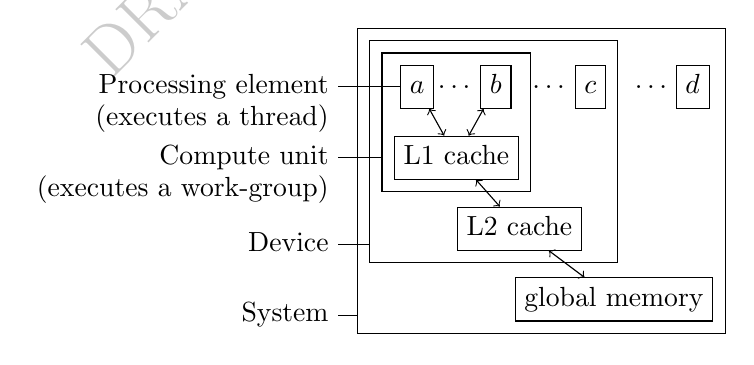
\begin{tikzpicture}[yscale=-1]
\node[draw] (T0) at (0,0) {\mystrut $a$};
\node at (0.5,0) {\dots};
\node[draw] (T1) at (1,0) {\mystrut $b$};
\node at (1.7,0) {\dots};
\node[draw] (T2) at (2.2,0) {\mystrut $c$};
\node at (3.0,0) {\dots};
\node[draw] (T3) at (3.5,0) {\mystrut $d$};
\node[anchor=east] (PE_lab) at (-1.0,0)
{\mystrut Processing element};
\node[anchor=east] (PE_lab2) at (-1.0,0.4)
{\mystrut (executes a thread)};

\node[draw] (L1) at (0.5,0.9) {\mystrut L1 cache};
\node[draw, fit=(T0)(T1)(L1), inner sep=1.5mm] (CU0) {};
\node[anchor=east] (CU_lab) at (-1.0,0.9)
{\mystrut Compute unit};
\node[anchor=east] (CU_lab2) at (-1.0,1.3)
{\mystrut (executes a work-group)};

\node[draw] (L2) at (1.3,1.8) {\mystrut L2 cache};
\node[draw, fit=(CU0)(T2)(L2), inner sep=1.5mm] (DV0) {};
\node[anchor=east] (DV_lab) at (-1.0,2.0) 
{\mystrut Device};

\node[draw] (G) at (2.5,2.7) {\mystrut global memory};

\node[draw, fit=(DV0)(T3)(G), inner sep=1.5mm] (SY0) {};
\node[anchor=east] (SY_lab) at (-1.0,2.9) 
{\mystrut System};

\draw[<->] (T0) to (L1);
\draw[<->] (T1) to (L1);
\draw[<->] (L1) to (L2);
\indirectline{T2}{L2}{6.5mm};
\draw[<->] (L2) to (G);
\indirectline{T3}{G}{6.5mm};

\draw[black] (SY_lab) to (SY0.west |- SY_lab);
\draw[black] (DV_lab) to (DV0.west |- DV_lab);
\draw[black] (CU_lab) to (CU0.west |- CU_lab);
\draw[black] (PE_lab) to (T0.west |- PE_lab);

\end{tikzpicture}
\caption{Illustration of the OpenCL execution hierarchy}
\label{fig:memory_scopes_example}
\end{figure}

\paragraph{Atomic operations} 
OpenCL 2.0 provides \emph{atomic operations}, which enable fine-grained lock-free synchronisation both within
and between work-groups and devices. The operations provide a range of
memory-consistency guarantees according to semantics defined by a
detailed C11-based \emph{memory model}~\cite[\S3.3]{munshi13}.
Operations with weaker guarantees may offer superior performance, but
have more subtle semantics.

\paragraph{Memory scopes} Where the OpenCL memory model departs
significantly from C11 is in its introduction of \emph{memory
scope} constants. The three constants are:
\[
\begin{array}{rlllll}
s ::= & \swg & \text{current work-group} \\
 \mid & \sdv & \text{current device} \\
 \mid & \sall & \text{all devices}
\end{array}
\] 
and, when attached to an atomic operation, govern how far through the
execution hierarchy the memory consistency guarantees must be
enforced. For instance, if a global memory location \texttt{x} is
currently being accessed only by threads in the same work-group, such
as $a$ and $b$ in Fig.~\ref{fig:memory_scopes_example}, the accesses can be scoped at $\swg$ so that they need travel no further than the L1 cache that $a$ and $b$ share.

Both participants in a synchronisation operation are required to use a
memory scope that is wide enough to encompass the other. This rule
would be violated if, for instance, thread $a$ in
Fig.~\ref{fig:memory_scopes_example} writes \texttt{x} at $\swg$
scope, thread $c$ (in a different work-group) reads \texttt{x}, and
there is no synchronisation in between. As we shall explain further in
\S\ref{sec:formalising_opencl}, such a situation is deemed by OpenCL
to be a \emph{race}: a programmer fault that renders the whole program
undefined.

\paragraph*{Work stealing} is a technique for achieving dynamic load
balancing in high-performance computing. In an OpenCL context, work
stealing involves each work-group owning a task queue, and idle
threads popping tasks from another work-group's queue should their
own queue become empty. The ability to steal work is valuable when it
is impractical to distribute tasks evenly among work-groups at
compile-time -- either because of a non-uniform computational cost per
task that depends on input data, or because new tasks can be created
dynamically at run-time~\cite{cederman+12}.

\paragraph{To scope or to steal?}
The current design of OpenCL allows programmers to exploit
work stealing, or to exploit the scoping mechanism, but not both. To
see this, consider an application that exploits scopes by having
threads use work-group scope when pushing to or popping from their
local task queue. This makes stealing impossible, regardless
of the stealer's scope, because synchronisation fails unless
\emph{both} of the operations that are synchronising use wide-enough
scopes. To make
stealing possible, we could arrange that every queue operation uses a
wider scope, but then we lose the benefit of using scopes: the common
case (accessing one's own queue) would take a performance hit to allow
the uncommon case (stealing from another's queue).

\paragraph{A solution: remote scope promotion}
Previous work proposed an extension to OpenCL's scoping mechanism~\cite{orr+15},
\emph{remote-scope promotion} (RSP), that \emph{is} compatible with
work stealing. It was shown that on a range of benchmarks from the Pannotia suite~\cite{che+13} (including Google's
PageRank), RSP combined with stealing leads to an average speedup of
17\% over scopes alone, and 6\% over stealing alone.

In OpenCL extended with RSP (OpenCL+RSP), each atomic
operation has an extra Boolean flag, indicating
whether the operation is \emph{remote}. In ordinary scoped
synchronisation, both of the synchronising operations must use
a wide-enough scope. The essence of RSP is to add another sufficient
condition for synchronisation; namely, that just one of the participants has a
wide-enough scope and is flagged as remote. In this case, the scope of
the other participant is irrelevant; it is silently promoted to match
the first participant's scope.

A mapping from OpenCL+RSP to hardware
primitives was described previously. Remote operations are compiled to special
instructions for flushing or invalidating caches that belong to other
work-groups or other devices. It was informally argued that the
implementation is correct. The implementation has been realised in a
simulator and has been tested using a number of examples.

\paragraph{The need for formality}
Like all new concurrency-related language constructs,
RSP has a subtle semantics that may be hard to implement correctly,
and is hard to reason about. (For instance, from the prose description
above: what should happen when \emph{both} participants in a pair of
synchronising operations are flagged as
remote?) Due to the inconclusive nature of testing, and the fundamental
problems associated with testing concurrent systems, we turn to formal
methods for a rigorous treatment of RSP.

\subsection{The OpenCL Memory Model}
\label{sec:formalising_opencl}

The OpenCL 2.0 memory model, which builds on the C11 memory model, is
the part of the OpenCL language specification that covers reading and
writing shared memory locations. It defines which values are allowed
to be read at a given program point, and whether two memory accesses
have a \emph{data race}. It is principally concerned with the
collection of \emph{atomic functions}, which can expose to programmers
the various \emph{weak memory} behaviours of the underlying hardware.
The C11 memory model was first formalised by Batty et
al.~\cite{batty+11}; this formalisation was then extended to the
OpenCL case by Wickerson et al.~\cite{wickerson+15}. In
\S\ref{sec:formalising_opencl+rsp}, we extend the memory model
further to formalise OpenCL+RSP.

\paragraph{Axiomatic memory models} All of these memory models are
defined \emph{axiomatically}. To define the set of a program's allowed
executions in this style, one first generates a superset thereof,
called the set of \emph{pre-executions}, which comprises those
executions that could be obtained with the use of a completely
non-deterministic memory that returns an arbitrary value for each
load. An `execution', in this context, comprises a set of run-time
memory events (such as $\evR_\sdv(\texttt{x},42)$, which indicates the
value $42$ being read from \texttt{x} using device scope), and several relations between
them (such as the \emph{program order} of the corresponding
instructions). One then whittles this down, using a set of axioms, to
the set of \emph{consistent} executions. A pre-execution is consistent
if it can be extended to a \emph{candidate
execution}\label{lab:candidate} that satisfies all of the axioms of
the memory model. A candidate execution additionally contains a
\emph{reads from} relation (representing data flow from write events
to read events) and a \emph{modification order} among the writes to
each location. These two relations together constitute the
\emph{execution witness}. If any of a program's candidate executions
is deemed to have a data race, the behaviour of the program is
\emph{undefined}, which means that it may behave arbitrarily (and the
behaviours of candidate executions that do not have data races become
irrelevant).

\paragraph{Syntax of OpenCL programs}
We restrict our attention to a small OpenCL-like language that
includes non-atomic loads and stores ($\texttt{load}_\na$ and
$\texttt{store}_\na$), scoped atomic acquire-loads and release-stores
($\texttt{load}_s$ and $\texttt{store}_s$), and a scoped `atomic
increment' operation ($\texttt{fetch\_inc}_s$) that demonstrates an
acquire+release RMW. Full OpenCL includes other varieties of atomic
memory access, such as relaxed and sequentially-consistent.

In real OpenCL, all threads execute the same
\emph{kernel program}, but can obtain differing control or data flows
by querying their own thread identifiers. In our simplified setting,
we suppose that each thread is programmed independently. Reflecting
the execution hierarchy in OpenCL, we formalise an
OpenCL program $P$ as a list of lists of lists of sequential programs:
\begin{eqnarray*}
P &::=& P_{\rm dv} \quadparallel \dots \quadparallel P_{\rm dv} \\
P_{\rm dv} &::=& P_{\rm wg} \tripleparallel \dots \tripleparallel P_{\rm
wg} \\
P_{\rm wg} &::=& p \parallel \dots \parallel p 
\end{eqnarray*}
where $p$ is a piece of sequential code, $\quadparallel$ separates
code executed by different devices, $\tripleparallel$ separates code
executed by different work-groups in the
same device, and $\parallel$ separates code executed by different
threads in the same work-group.

\begin{Example} 
\label{ex:rmw_atomicity}
The following program comprises two threads in two different
work-groups on the same device.
\[
\begin{array}{l|||l}
\texttt{fetch\_inc}_\sdv(\texttt{x}) & 
\texttt{store}_\sdv(\texttt{x}, 2)
\end{array}
\]
One thread increments \texttt{x} and the other sets \texttt{x} to
2. The use of $\sdv$-scope for both operations ensures that these
conflicting accesses do not race.
\end{Example}

\subsection{Details of the Memory Model}

\begin{figure}
\renewcommand\FrameSep{1mm}
\newcommand\myskip{\vspace*{1.5mm}}
\begin{shaded}
\newcommand\figureheading[1]{\textbf{#1:}}
 \figureheading{Location types}~~Each location is atomic or non-atomic
\par\medskip
\figureheading{Event labels} For locations $x$, scopes $s$, and values $v$:
\begin{itemize}[topsep=0pt, noitemsep]
\item $\evWna(x,v)$\,/\,$\evRna(x,v)$: non-atomic
write/read 
\item $\evW_{s}(x,v)$\,/\,$\evR_{s}(x,v)$: atomic write/read
\item $\evRMW_{s}(x,v,v')$: atomic read-modify-write
\end{itemize}
\par\myskip
\figureheading{Predefined subsets of events}
\begin{itemize}[topsep=0pt, noitemsep]
\item $R$: the set of read and RMW events
\item $W$: the set of write and RMW events
\item $I$: the set of initialisation events (each a non-atomic write of
$0$, one per location)
\item $\naL$: events that access a non-atomic location
\item $\na$: non-atomic events
\item $\swg$\,/\,$\sdv$\,/\,$\sall$: the set of events that are parameterised by the
respective memory scope
\end{itemize}
\myskip
\figureheading{Primitive relations}
\begin{itemize}[topsep=0pt, noitemsep]
\item $\thd$/$\wg$/$\dv$: an equivalence relation over all
(non-initialisation) events, relating events from the same thread/work-group/device
\item $\loc$: an equivalence relation over all events, relating events that access
the same location
\item $\Sb$ (sequenced before): a strict partial order specifying
the order of each thread's instructions, and also linking initialisation events to non-initialisation events
\item $\rf$ (reads from): contained in $W \times R$, relating writes to
reads when the locations and values match, each read reads from
exactly one write
\item $\mo$ (modification order): a strict partial order that relates
all and only writes to the same
atomic
location
\end{itemize}
\myskip
\figureheading{Derived relations}
\begin{itemize}[topsep=0pt, noitemsep]
\item $\var{rs'} \eqdef \thd \cup (\unv ; [R \cap W])$
\item $\var{rs} \eqdef \mo \cap \var{rs'} \setminus ((mo \setminus \var{rs'}) ; \mo)$
\item $\var{incl1} \eqdef ([\swg] ; \wg) \cup ([\sdv] ; \dv) \cup
([\sall] ; \unv)$
\item $\var{incl} \eqdef \var{incl1} \cap \var{incl1}^{-1}$
\item $\var{sw} \eqdef ([W\setminus\na] ; \var{rs}^? ; \rf ; [R\setminus\na]) \cap \var{incl} \setminus \thd$
\item $\hb \eqdef (\Sb \cup
\var{sw})^+$
\item $\var{hbl} \eqdef \var{hb} \cap \loc$
\item $\var{vis} \eqdef \var{hb} \setminus (\var{hb} ; [W] ; \var{hbl})$
\item $\var{conflict} \eqdef ((W \times W) \cup (W \times R) \cup (R
\times W)) \cap \loc$ 
\item $\var{dr} \eqdef \var{conflict} \setminus \hb \setminus \hb^{-1} \setminus \var{incl}$
\end{itemize}
\myskip
\figureheading{Consistency axioms}
\par\centering
\renewcommand\arraystretch{1.2}
\begin{tabular}{@{}p{82mm}@{}}
$\irreflexive (\hb) \hfill \Tag{\axiom{Hb}}$
\\
$\irreflexive ((\rf^{-1})^? ; \mo ;
\rf^? ; \hb) \hfill
\Tag{\axiom{Coh}}$
\\
$\irreflexive (\rf ; \hb) \hfill
\Tag{\axiom{Rf}}$
\\
$\isempty ((\rf ; [\naL]) \setminus \var{vis}) \hfill \Tag{\axiom{Narf}}$
\\
$\irreflexive (\rf \cup (\mo ; \mo ; \rf^{-1})
\cup (\mo ; \rf)) \hfill \Tag{\axiom{Rmw}}$
\end{tabular}
\par\raggedright
\myskip
\figureheading{Non-faultiness axiom}
\par\centering
\begin{tabular}{@{}p{82mm}@{}}
$\isempty(\var{dr}) \hfill \Tag{\axiom{Dr}}$
\end{tabular}
\end{shaded}
\caption{The OpenCL memory model (simplified)}
\label{fig:openclmm}
\end{figure}

The details of the OpenCL memory model are summarised in
Fig.~\ref{fig:openclmm}. We give the language from which event labels
are drawn -- this ranges over read ($\mathrm{R}$), write
($\mathrm{W}$), and read-modify-write ($\mathrm{RMW}$) events (which
represent, for instance, an atomic increment or a successful
compare-and-swap). We provide identifiers for particular subsets of
events in any given candidate execution, and list the basic and
derived relations between events. We finally give the axioms of the
memory model, following the \cat{} format of Alglave et
al.~\cite{alglave+14}. Five axioms (the consistency
axioms) characterise consistent executions, and one further axiom (the
non-faultiness axiom) characterises the absence of data races. We
shall explain these axioms further, after introducing the following
notational conventions.

\begin{Notation}
We write $r^+$ for the transitive closure of a relation $r$, $r^{-1}$
for its inverse, and we abbreviate $r\cup\var{id}$ as $r^{?}$, where
$\var{id}$ is the identity relation. We write $\neg$ for complement,
$\setminus$ for set difference,
$\unv$ for the universal relation, and $[s]$ to abbreviate
$\{(x,x)\mid x\in s\}$. We define relational composition ($;$) such
that $(x,z)\in r_1; r_2$ if $(x,y)\in r_1$ and $(y,z)\in r_2$ for some
$y$. (This notation is convenient for describing shapes in execution
graphs; for instance, the relation $[s_1];r_1;[s_2];r_2;[s_3]$ relates
events in $s_1$ to those in $e_3$ that can be reached by taking an
$r_1$-edge to an event in $s_2$ and then taking an $r_2$-edge.)
\end{Notation}

The $\var{rs}'$ and $\var{rs}$ relations define the \emph{release
sequence}, which is inherited without modification from C11 and can be
safely ignored by the unfamiliar reader. The $\var{incl1}$ relation
connects event $e_1$ to event $e_2$ whenever $e_1$'s scope is no
narrower than the distance between the events in the execution
hierarchy at run-time. When this relation also holds in the opposite
direction ($\var{incl}^{-1}$), then the events are deemed to have
inclusive scopes, as captured by the $\var{incl}$
relation. Inter-thread synchronisation ($\var{sw}$,
`synchronises-with') relates an atomic write to an atomic read in another thread that
reads from it, providing the two events have inclusive
scopes. Happens-before ($\var{hb}$) edges are induced both by the
program order and by synchronisation. They must not form cycles
(\axiom{Hb}); that is, the shape \smash{\begin{tikzpicture}[baseline=-1mm,inner sep=1pt]
\node (a) at (0,0) {};
\draw[edgehb] (a) to [auto, swap, out=-30, in=30, min distance=15] (a);
\end{tikzpicture}}\hspace{-2pt}\textcolor{colorhb}{$\var{hb}$} is forbidden. 

The principle of \emph{coherence}~(\axiom{Coh}) governs the relationship between
$\var{hb}$ and $\var{mo}$: if the write $w_1$ is $\var{mo}$-before the
write $w_2$, then $w_2$ (and any events that read from $w_2$) must not
happen before $w_1$ (nor before any events that read from
$e_1$). Coherence forbids the following shapes.
%
\begin{center}
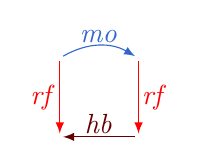
\begin{tikzpicture}[inner sep=1pt, baseline=2mm]
\node (a) at (1,1) {};
\node (b) at (0,1) {};
\node (c) at (0,0) {};
\node (d) at (1,0) {};
\draw[edgemo] (b) to [auto, bend left] node {$\var{mo}$} (a);
\draw[edgerf] (b) to [auto, swap] node {$\var{rf}$} (c);
\draw[edgehb] (d) to [auto, swap] node {$\var{hb}$} (c);
\draw[edgerf] (a) to [auto] node {$\var{rf}$} (d);
\end{tikzpicture}
~
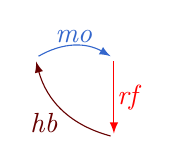
\begin{tikzpicture}[inner sep=1pt, baseline=2mm]
\node (a) at (1,1) {};
\node (b) at (0,1) {};
\node (d) at (1,0) {};
\draw[edgemo] (b) to [auto, bend left] node {$\var{mo}$} (a);
\draw[edgehb] (d) to [auto, bend left] node {$\var{hb}$} (b);
\draw[edgerf] (a) to [auto] node {$\var{rf}$} (d);
\end{tikzpicture}
~
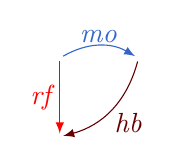
\begin{tikzpicture}[inner sep=1pt, baseline=2mm]
\node (a) at (1,1) {};
\node (b) at (0,1) {};
\node (c) at (0,0) {};
\draw[edgemo] (b) to [auto, bend left] node {$\var{mo}$} (a);
\draw[edgerf] (b) to [auto, swap] node {$\var{rf}$} (c);
\draw[edgehb] (a) to [auto, bend left] node {$\var{hb}$} (c);
\end{tikzpicture}
~
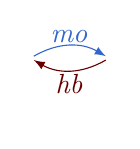
\begin{tikzpicture}[inner sep=1pt, baseline=2mm]
\node (a) at (1,1) {};
\node (b) at (0,1) {};
\draw[edgemo] (b) to [auto, bend left] node {$\var{mo}$} (a);
\draw[edgehb] (a) to [auto, bend left] node {$\var{hb}$} (b);
\end{tikzpicture}
\end{center}

The reads-from axiom (\axiom{Rf}) forbids reads to observe writes
that happened after them (\textcolor{colorhb}{$\var{hb}$}\,
\begin{tikzpicture}[inner sep=1pt, baseline=0.3em]
\node (a) at (0,0) {};
\node (b) at (0,1.2em) {};
\draw[edgerf] (a) to [auto, swap, bend right] (b);
\draw[edgehb] (b) to [auto, swap, bend right] (a);
\end{tikzpicture}\,\textcolor{colorrf}{$\var{rf}$}).
%
The non-atomic reads-from axiom (\axiom{Narf}) requires non-atomic reads
to observe an immediate predecessor in $\var{hb}$, called a
\emph{visible write}: i.e. we must
have
\textcolor{colorhb}{$\var{hb}$}\,
\begin{tikzpicture}[inner sep=1pt, baseline=0.3em]
\node (a) at (0,0) {};
\node (b) at (0,1.2em) {};
\draw[edgerf] (b) to [auto, swap, bend left] (a);
\draw[edgehb] (b) to [auto, swap, bend right] (a);
\end{tikzpicture}\,\textcolor{colorrf}{$\var{rf}$}
but no $\var{hb}$-intervening write to the same location $\left(
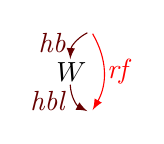
\begin{tikzpicture}[inner sep=1pt, baseline=(r.base)]
\node (a) at (0,0) {};
\node (b) at (-0.7em,1.5em) {$W$};
\node (c) at (0,3.0em) {};
\draw[edgerf] (c) to [auto, bend left] node (r) {$\var{rf}$} (a);
\draw[edgehb] (c) to [auto, swap, bend right,pos=0.9] node {$\var{hb}$} (b);
\draw[edgehb] (b) to [auto, swap, bend right, pos=0.1] node {$\var{hbl}$} (a);
\end{tikzpicture}\hspace{-1mm}\right)$.

The principle of \emph{RMW atomicity} (\axiom{Rmw}) dictates that each
RMW event must observe the $\mo$-latest write to that location; that
is, it must not observe itself (\smash{\begin{tikzpicture}[baseline=-1mm,inner sep=1pt]
\node (a) at (0,0) {};
\draw[edgerf] (a) to [auto, swap, out=-30, in=30, min distance=15] (a);
\end{tikzpicture}}\hspace{-2pt}\textcolor{colorrf}{$\var{rf}$}), it must not observe a write that is too late (\textcolor{colormo}{$\var{mo}$}\hspace{1pt}
\begin{tikzpicture}[inner sep=1pt, baseline=0.3em]
\node (a) at (0,0) {};
\node (b) at (0,1.2em) {};
\draw[edgerf] (a) to [auto, swap, bend right] (b);
\draw[edgemo] (b) to [auto, swap, bend right] (a);
\end{tikzpicture}\hspace{1pt}\textcolor{colorrf}{$\var{rf}$}), and it
must not observe a write that is
too early $\left(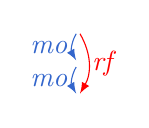
\begin{tikzpicture}[inner sep=1pt, baseline=(r.base)]
\node (a) at (0,0) {};
\node (b) at (0,1.2em) {};
\node (c) at (0,2.4em) {};
\draw[edgerf] (c) to [auto, bend left] node (r) {$\var{rf}$} (a);
\draw[edgemo] (c) to [auto, swap, bend right] node {$\var{mo}$} (b);
\draw[edgemo] (b) to [auto, swap, bend right] node {$\var{mo}$} (a);
\end{tikzpicture}\hspace{-1mm}\right)$. 

Finally, an execution has a data race ($\var{dr}$) if two conflicting
events are unrelated by happens-before and do not have inclusive
scopes. The non-faultiness axiom (\axiom{Dr}) detects data races.


\begin{Example} 
\label{ex:rmw_atomicity_2}
Here are two executions of the program in
Example~\ref{ex:rmw_atomicity}, both of which satisfy all of the
consistency axioms and the non-faultiness axiom. The initial event is
drawn above the events of the two parallel threads. Reflexive and
transitive edges are elided.  The left-hand execution gives rise to
the final state $\texttt{x}=2$, while the right-hand one finishes with $\texttt{x}=3$.
%
\begin{center}
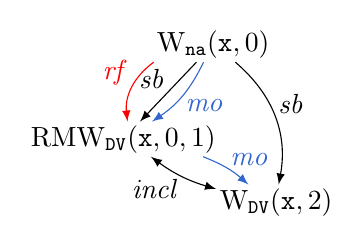
\begin{tikzpicture}[inner sep=1pt]
\node[event, anchor=west](a) at (0.4,2)
{$\evWna({\tt x},0)$};

\node[event, anchor=west](b) at (-1.2,0.8) 
{$\evRMW_{\sdv}(\texttt{x},0,1)$};

\node[event, anchor=west](c) at (1.2,0) 
{$\evW_{\sdv}(\texttt{x},2)$};

\draw[edgerf] (a) to[auto, swap, bend right=30] 
node {$\var{rf}$} (b);

\draw[edgesb] (a) to [auto, swap] node {$\var{sb}$} (b);

\draw[edgemo] (a) to[auto, bend left=15] 
node {$\var{mo}$} (b);

\draw[edgemo] (b) to[auto, bend left=10] node {$\var{mo}$} (c);

\draw[edgethd] (b) to[auto,swap, bend right=10] node {$\var{incl}$} (c);

\draw[edgesb] (a) to[auto, bend left] node {$\var{sb}$} (c);
\end{tikzpicture}
\hfill
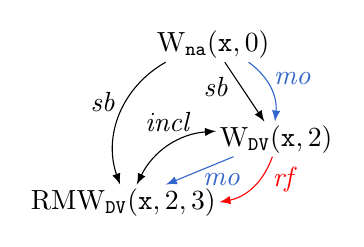
\begin{tikzpicture}[inner sep=1pt]
\node[event, anchor=west](a) at (0.4,2)
{$\evWna({\tt x},0)$};

\node[event, anchor=west](b) at (-1.2,0) 
{$\evRMW_{\sdv}(\texttt{x},2,3)$};

\node[event, anchor=west](c) at (1.2,0.8) 
{$\evW_{\sdv}(\texttt{x},2)$};

\draw[edgerf] (c) to[auto, bend left, pos=0.1] node
{$\var{rf}$} (b.east);

\draw[edgesb] (a) to [auto, swap, bend right=40] node {$\var{sb}$} (b);

\draw[edgemo] (a) to[auto, bend left] 
node {$\var{mo}$} (c);

\draw[edgesb] (a) to[auto, swap,pos=0.2] node {$\var{sb}$} (c);

\draw[edgemo] (c) to[auto] node {$\var{mo}$} (b);

\draw[edgethd] (b) to[auto, bend left, pos=0.8] node {$\var{incl}$} (c);
\end{tikzpicture}
\end{center}
Other final values for \texttt{x} are not allowed. For instance, the
following execution, which would result in $\texttt{x}=1$, falls foul
of the \axiom{Rmw} axiom: it constitutes a violation of RMW atomicity.
\begin{center}
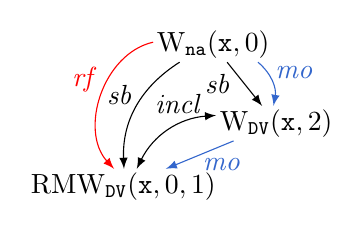
\begin{tikzpicture}[inner sep=1pt]
\node[event, anchor=west](a) at (0.4,2)
{$\evW_{\na}({\tt x},0)$};

\node[event, anchor=west](b) at (-1.2,0.2) 
{$\evRMW_{\sdv}(\texttt{x},0,1)$};

\node[event, anchor=west](c) at (1.2,1) 
{$\evW_{\sdv}(\texttt{x},2)$};

\draw[edgerf] (a) to[auto, swap, bend right=60] node
{$\var{rf}$} (b);

\draw[edgesb] (a) to [auto, swap, bend right] node {$\var{sb}$} (b);

\draw[edgemo] (a) to[auto, bend left] 
node {$\var{mo}$} (c);

\draw[edgesb] (a) to[auto, swap,pos=0.2] node {$\var{sb}$} (c);

\draw[edgemo] (c) to[auto] node {$\var{mo}$} (b);

\draw[edgethd] (b) to[auto, bend left, pos=0.9] node {$\var{incl}$} (c);
\end{tikzpicture}
\vspace*{-6mm}
\end{center}
\end{Example}

\begin{Example}
\label{ex:rmw_atomicity_3}
If the program in Example~\ref{ex:rmw_atomicity} were changed so that
the increment had work-group scope:
\[
\begin{array}{l|||l}
\texttt{fetch\_inc}_\swg(\texttt{x}) & 
\texttt{store}_\sdv(\texttt{x}, 2)
\end{array}
\]
then the scope-inclusion ($\var{incl}$) edges seen in Example~\ref{ex:rmw_atomicity_2}
would all be replaced with data race
($\var{dr}$) edges.
\end{Example}

\paragraph{Simplifications and other discrepancies with the standard}
We do not consider the distinction between global memory (shared among
all threads) and local memory (shared among threads in a work-group),
and instead treat all memory as global; local memory is not
interesting in the context of memory scopes, since the only allowable
scope with which local memory can be accessed atomically is $\swg$. Fences, barriers, relaxed atomics, and
sequentially-consistent atomics were not discussed in previous work on
RSP~\cite{orr+15} and are largely orthogonal.

OpenCL employs a stricter form of scope inclusion, in
which both events must additionally use the \emph{same} memory scope.
The version we use here follows a proposal called
HRF-relaxed~\cite{gaster+15}, and is a necessary prerequisite for RSP.

\section{Formalising OpenCL+RSP}
\label{sec:formalising_opencl+rsp}

We now describe our first research contribution: how to extend the
OpenCL memory model with RSP. The purpose of this extension is: (a) to
enable programs that exploit RSP to be analysed
(\S\ref{sec:testing}), and (b) to enable a proof that the
implementation of the language features is correct (\S\ref{sec:implementation}). Note
that (b) is an important enabler for (a), because the program analysis
would be meaningless were the OpenCL+RSP memory model impossible to
implement.

Adding RSP to OpenCL first involves extending the syntax of the
language, and to this end, we propose simply to add an additional
parameter to each existing atomic function, which accepts either
\texttt{N} (for non-remote) or \texttt{R} (for remote) -- see
Example~\ref{ex:rmw_atomicity_4} below. Second, we
must extend the semantics of the language (i.e., the memory model). This
requires changing just one definition, the $\var{incl}$ relation in Fig.~\ref{fig:openclmm}, as follows:
\[
\var{incl} \eqdef \stack{\var{incl1} \cap \var{incl1}^{-1} \\ \mhl{{}\cup
([\var{rem}]; \var{incl1}) \cup
(\var{incl1}^{-1}; [\var{rem}])}}
\]
where $\var{rem}$ identifies the set of events representing a remote
operation. In the original definition, both events must have wide
enough scopes; in the new version, the events (say $e_1$ and $e_2$)
may \emph{also} synchronise if $e_1$'s scope is wide enough to reach
$e_2$ and $e_1$ is remote, or if $e_2$'s scope is wide enough to reach
$e_1$ and $e_2$ is remote.\footnote{We initially sought to encode RSP
by instead adding an extra disjunct to the $\var{incl1}$ relation:
$\var{incl1} \eqdef \ldots \cup ([\var{rem}];\unv)$. Although
seductively simple, this version does not capture the intended
behaviour of RSP in the case where \emph{both} participants are marked
remote; rather, it would erroneously allow two remote $\swg$-scoped
operations to synchronise across different devices.}

\begin{Example}
\label{ex:rmw_atomicity_4}
If the program in Example~\ref{ex:rmw_atomicity_3} were changed so that
the store became \emph{remote}:
\[
\begin{array}{l|||l}
\texttt{fetch\_inc}_{\swg,\texttt{N}}(\texttt{x}) & 
\texttt{store}_{\sdv,\texttt{R}}(\texttt{x}, 2)
\end{array}
\]
then the scope-inclusion ($\var{incl}$) edges seen in the executions in
Example~\ref{ex:rmw_atomicity_2} would be restored.
\end{Example}

The simple manner in which we can adapt the memory model for RSP
illustrates the elegance of an axiomatic memory model. Our extension
is conservative in the sense that it does not affect the semantics of
OpenCL programs that do not exploit RSP. It is significantly simpler
than a previous outline formalisation~\cite{orr+15}, and is further distinguished by being
founded on an existing, comprehensive
formalisation of OpenCL~\cite{wickerson+15}. Although the details of
implementing RSP are rather involved (as we discuss in detail in
\S\ref{sec:implementation}), the effect of RSP on the memory model is
minimal. The minor modification to the $\var{incl}$ relation is all
that is required to enable simulation of litmus tests that exploit
RSP, which we discuss next.

\section{Testing OpenCL+RSP Programs}
\label{sec:testing}

We extended the memory model simulator \herd{} to support the
simulation of small OpenCL+RSP programs against the newly-extended
memory model (\S\ref{sec:extending_herd}). We then used
\herd{} to analyse a suite of test
programs that we obtained from the broader group of original RSP developers, uncovering
several faults in the process (\S\ref{sec:litmus_testing}), and
further exercised \herd{} to debug a larger OpenCL+RSP
application: a work-stealing queue (\S\ref{sec:work_stealing}).

\subsection{Extending \herd{}}
\label{sec:extending_herd} 

\Herd{} is a generic memory model simulator~\cite{alglave+14}. Its
basic operation is to generate and iterate through a set of candidate
executions of a given litmus test, and assess whether each is
consistent and/or faulty according to the axioms of a given memory
model, as described using the \cat{} specification language.
Originally designed for CPU assembly programs~\cite{alglave+14},
\herd{} has recently been extended with the capacity to simulate C11
and OpenCL programs~\cite{wickerson+15}. For the current work, we have
extended \herd{} further, to support OpenCL+RSP. This entailed two
sub-tasks: extending the front end of \herd{} to understand remote
versions of atomic operations in litmus tests, and extending the
memory model specification language with an additional identifier,
$\var{rem}$, to stand for the set of remote events in an execution.

\subsection{Litmus Testing}
\label{sec:litmus_testing}

The original developers of RSP used a suite of 12 litmus tests to
gain confidence in the correctness of their implementation. These
tests, which are mostly variants on standard litmus tests,
characterise the building blocks of parallel algorithms that use RSP.
We obtained the suite from the RSP developers, and used \herd{} to
simulate each test against our formalisation of the OpenCL+RSP memory
model.

\paragraph{Preparation} 
We encoded each program into the \texttt{.litmus} format that is
accepted by \herd{}. In doing so, we observed that the
original litmus tests make several uses of empty loops that spin until
a given location holds a specific value, such as `\texttt{while
(load(x) != 1); C}'. Because such programs have arbitrarily-many
candidate executions (one for each possible iteration count) we
followed standard practice in preparing litmus tests (
e.g., Alglave et al.~\cite{alglave+15}) and replaced the pattern above with
`\texttt{if (load(x) == 1) \{C\}}', ignoring those executions where
the conditional test failed.

\paragraph{Results}
We performed simulation on a 2.8~GHz MacBook Pro, and observed that
each litmus test was fully simulated in less than one second, except
for two tests that made use of several compare-exchange instructions;
each of these tests was fully simulated in less than three minutes.

Seven of the 12 litmus tests included postconditions on the final
state of memory that we found, through analysis with \herd{}, to be
satisfied by all consistent executions.  Another test exhibited a
deliberate data race that was confirmed by \herd{}.

Our analysis exposed bugs in the other four litmus tests. The
first test had an unintentional data race, resulting from a
discrepancy between the HSA 1.0 memory model~\cite{kyriazis+12} and
the OpenCL 2.0 memory model. Specifically, OpenCL does not enforce
happens-before between two operations that access different regions of
memory even if they belong to the same thread,
so one cannot
assume the HSA behaviour, which does enforce happens-before here.
The second test also contained a data race. The third had an incorrect postcondition due to a simple arithmetic
error. The fourth had a postcondition that was too strong: it forbade
certain executions that were allowed by the axioms of the memory
model. As it happens, the proposed implementation does not give rise
to the executions that this litmus test forbids; it can therefore be
deemed a conservative implementation of the OpenCL specification in
this regard.

\subsection{Case Study: A Work-Stealing Queue}
\label{sec:work_stealing}

We used \herd{} to probe the correctness of a more realistic
OpenCL+RSP application: a work-stealing queue. This application,
is a key motivator for RSP~\cite[\S3.2]{orr+15}, and exploits RSP by simultaneously optimising
for the common case of accessing the local task queue (by using
$\swg$-scoped non-remote operations in \texttt{push} and \texttt{pop})
and enabling the uncommon case of accessing a different work-group's
queue (by using $\sdv$-scoped remote operations in \texttt{steal}).

Alglave et al.~\cite{alglave+15} have uncovered two bugs in a similar
CUDA implementation~\cite{cederman+12} that led to tasks occasionally
being dropped from queues; both bugs arose from assuming an
overly-strong memory model. This was demonstrated by hand-compiling
suspect slices of the CUDA code into GPU assembly litmus tests (named
\emph{dlb-mp} and \emph{dlb-lb}) and showing experimentally that these
tests could produce results that would lead to bugs at the CUDA level.

We have been able to demonstrate the complementary result for the
OpenCL+RSP work-stealing queue. We produced OpenCL+RSP litmus tests
capturing the same thread interactions that \emph{dlb-mp} and
\emph{dlb-lb} captured at the GPU assembly level. Using \herd{}, we
were able to verify the \emph{absence} of the bugs associated with the
original CUDA implementation, thanks to sufficient use of
store-release and load-acquire functions to ensure necessary
synchronisation. Because our result demonstrates correctness at the
level of the programming language, it extends to \emph{any} correct
implementation of OpenCL+RSP.

We emphasise that we have not verified the entirety of the
work-stealing queue implementation; we merely state that it is free
from two specific bugs. Indeed, on the contrary, we found,
reported, and confirmed a data race that could arise when performing a \texttt{pop}
and a \texttt{steal} on the same queue. The race, which arises because
\texttt{pop} can non-atomically write to the queue's tail pointer
while the \texttt{steal} atomically reads from it, can be rectified by
upgrading the non-atomic write to a relaxed atomic write.


\section{A Formalised Implementation of OpenCL+RSP}
\label{sec:implementation}

Having studied the programming language semantics of RSP,
we now turn our attention to
formalising a low-level implementation of RSP, transforming the published description of the implementation of
OpenCL+RSP into rigorous mathematics.
%
Our formalisation comprises a mathematical model of a simple GPU device
(\S\ref{sec:hardware_model}), the syntax and semantics of a minimal
assembly language for this device (\S\ref{sec:assembly_language} and \S\ref{sec:environmental_transitions})
and a scheme for compiling OpenCL+RSP to assembly
(\S\ref{sec:compilation_scheme} and \S\ref{sec:problems_compilation_scheme}).

Our formalisation effort 
found several opportunities to improve the original compilation scheme,
ranging from improving inefficiencies to eliminating errors.
Our revised compilation scheme is simpler than the original and addresses
all of the errors and inefficiencies we found, hence we present the revised scheme first
(\S\ref{sec:compilation_scheme}), then explain
the original scheme in terms of how it differs from our proposal
(\S\ref{sec:problems_compilation_scheme}). In \S\ref{sec:soundness} we prove that our revised scheme is sound.

\paragraph{Tool support from Isabelle}
The definitions in this section have been formalised using the
Isabelle proof assistant~\cite{nipkow+02}, and the scripts are
available in our online companion material. We have also formalised
the statement of our soundness theorem (Thm.~\ref{thm:soundness},
\S\ref{sec:soundness}), but have not mechanised its proof. We found
the type-checking and custom syntax that Isabelle provides to be
invaluable while designing our model. We remark that the semantics of
assembly instructions (\S\ref{sec:assembly_language}), each of which
updates various components in a deeply-nested structure of records and
lists, is naturally expressed in an imperative style; because Isabelle
demands a functional style, our formalisation differs in this respect
from the current presentation.


\subsection{A Model of GPU Hardware}
\label{sec:hardware_model}

Our model of GPU hardware closely resembles the illustration in
Fig.~\ref{fig:memory_scopes_example}, which in turn is based on the model used for the original design of RSP~\cite[Fig.~4]{orr+15}.

\begin{figure*}
\subfloat[Formal definitions]{
$\begin{array}{@{}r@{~}c@{\hspace{-5.5mm}}r@{~~}c@{~~}l@{}}
x &\in& \var{Loc} \\
r &\in& \var{Reg} \\
v &\in& \var{Val} &\eqdef& \mathbb{Z} \\
&& \var{FifoEl} &\eqdef& \var{Loc} \cup
\{\textsc{flush}_{d,w,t}\mid d,w,t\in\mathbb{N}\} 
\\
&& \var{Fifo} &\eqdef& \var{FifoEl}\,\mathrm{queue}
\\
&& \var{Hygiene} &\eqdef& \{\CLEAN,\DIRTY\}
\\
&& \var{Freshness} &\eqdef& \{\VALID,\INVALID\}
\\
&& \var{CacheEntry} &\eqdef& \var{Val} \times
(\mathrm{hy}{:}\,\var{Hygiene}) \times (\mathrm{fr}{:}\,\var{Freshness})
\\
C &\in& \var{Cache} &\eqdef& (\var{Loc} \rightharpoonup\var{CacheEntry}) \times (\mathrm{fifo}{:}\,\var{Fifo})
\\
l &\in& \var{Lock} &\eqdef& \{\text{\unpadlock}\} \cup
\{\text{\padlock{d,w,t}}\mid d,w,t \in \mathbb{N}\}
\\
&& \var{ThState} &\eqdef& \var{Reg} \rightarrow \var{Val}
\\
&& \var{WgState} &\eqdef& \var{ThState}\,\mathrm{list} \times
(\mathrm{L1}{:}\, \var{Cache}) \times (\mathrm{rmw}{:}\,\var{Lock})
\\
&& \var{DvState} &\eqdef& \stack{\var{WgState}\,\mathrm{list} \times
(\mathrm{L2}{:}\,\var{Cache}) \times {}\\{} (\mathrm{lockfile}{:}\,\var{Loc} \rightarrow \var{Lock})}
\\
&& \var{Global} &\eqdef& \var{Loc} \rightharpoonup \var{Val} 
\\
\Sigma &\in& \var{SyState} &\eqdef& \var{DvState}\,\mathrm{list} \times (\mathrm{gl}{:}\,\var{Global})
\end{array}$
\label{fig:states}
}
\hfill
\subfloat[A machine state $\Sigma$, pictorially]{
\pgfdeclarelayer{john1}
\pgfdeclarelayer{john2}
\pgfdeclarelayer{john3}
\pgfsetlayers{background,john1,john2,john3,main}
\begin{tikzpicture}[yscale=-1, baseline=-11.5mm]
\small
\newcommand\mrot[1]{\rotatebox{90}{$#1$}}

\node (regfile) at (0,0) {
$\begin{array}{@{}l@{~}|@{~}l@{}}
%\hline
\mrot{\var{Reg}} & \mrot{\var{Val}} \\ 
\hline \rule{0mm}{2mm} \\ 
%\hline
\end{array}$};

\node[above=2mm of regfile.north west, anchor=west, inner sep=0] (pestate_lab) {$\var{ThState}$};

\begin{pgfonlayer}{john3}
\node[draw, rounded corners, fit = (regfile) (pestate_lab), xshift=1mm, yshift=1mm] {}; 

\node[draw, rounded corners, fit = (regfile) (pestate_lab), xshift=0.5mm, yshift=0.5mm] {}; 

\node[draw, fill=white, rounded corners, outer sep=1mm, fit = (regfile) (pestate_lab)] (pestate) {}; 
\end{pgfonlayer}

%\node[right=2mm of pestate] (pestate_dots) {};

\node[draw, rounded corners, below=0mm of pestate.south west,
anchor=north west, outer sep=1mm] (rmwlock)
{$\mathrm{rmw}{:}\,\var{Lock}$};

\node[right=10mm of regfile.north east, anchor=north west, yshift=4mm] (l1store) {
$\begin{array}{@{}l@{~}|@{~}l@{~}|@{~}l@{~}|@{~}l@{}}
%\hline
\mrot{\var{Loc}} & \mrot{\var{Val}} & \mrot{\var{Hygiene}} & \mrot{\var{Freshness}} \\ 
\hline
~ & ~ & ~ & ~ \\ 
%\hline
\end{array}$};

\node[above=2mm of l1store.north west, anchor=west, inner sep=0] (l1cache_lab)
{$\mathrm{L1}{:}\,\var{Cache}$};

\node[draw, rounded corners, below=0mm of l1store.south west, anchor=north west, outer sep=1mm] (l1fifo)
{$\mathrm{fifo}{:}\,\var{Fifo}$};

\node[draw, rounded corners, outer sep=1mm, fit = (l1store) (l1cache_lab) (l1fifo)] (l1cache) {}; 

\node[above=1mm of pestate.north west, anchor=south west, inner sep=0] (custate_lab)
{$\var{WgState}$};

\begin{pgfonlayer}{john2}
\node[draw, rounded corners, fit = (pestate) (rmwlock) (l1cache) (custate_lab), xshift=1mm, yshift=1mm, outer sep=1mm] (custate_shadow) {};

\node[draw, rounded corners, fit = (pestate) (rmwlock) (l1cache) (custate_lab), xshift=0.5mm, yshift=0.5mm, outer sep=1mm] {};

\node[draw, fill=white, rounded corners, fit = (pestate) (rmwlock) (l1cache) (custate_lab), outer sep=1mm]
(custate) {};
\end{pgfonlayer}

\node[right=34mm of regfile.north east, anchor=north west, yshift=10mm] (l2store) {
$\begin{array}{@{}l@{~}|@{~}l@{~}|@{~}l@{~}|@{~}l@{}}
%\hline
\mrot{\var{Loc}} & \mrot{\var{Val}} & \mrot{\var{Hygiene}} & \mrot{\var{Freshness}} \\ 
\hline
~ & ~ & ~ & ~ \\ 
%\hline
\end{array}$};

\node[above=2mm of l2store.north west, anchor=west, inner sep=0] (l2cache_lab)
{$\mathrm{L2}{:}\,\var{Cache}$};

\node[draw, rounded corners, below=0mm of l2store.south west, anchor=north west, outer sep=1mm] (l2fifo)
{$\mathrm{fifo}{:}\,\var{Fifo}$};

\node[draw, rounded corners, outer sep=1mm, fit = (l2store) (l2cache_lab) (l2fifo)] (l2cache) {}; 

\node[below=5mm of l2cache.south west, anchor=north west, xshift=2mm] (lockfile_store) {
$\begin{array}{@{}l@{~}|@{~}l@{}}
%\hline
\var{Loc} & \var{Lock} \\ 
\hline 
~ & ~ \\ 
%\hline
\end{array}$};

\node[above=2mm of lockfile_store.north west, anchor=west, inner sep=0] (lockfile_lab)
{$\mathrm{lockfile}$};

\node[draw, rounded corners, fit = (lockfile_store) (lockfile_lab), outer sep=1mm] (lockfile) {};

\node[above=1mm of custate.north west, anchor=south west, inner sep=0] (dvstate_lab)
{$\var{DvState}$};

\begin{pgfonlayer}{john1}
\node[draw, rounded corners, fit = (custate) (dvstate_lab) (custate_shadow) (l2cache) (lockfile), xshift=1mm, yshift=1mm, outer sep=1mm] (dvstate_shadow)
{};

\node[draw, rounded corners, fit = (custate) (dvstate_lab) (custate_shadow) (l2cache) (lockfile), xshift=0.5mm, yshift=0.5mm, outer sep=1mm] {};

\node[draw, fill=white, rounded corners, fit = (custate) (dvstate_lab) (custate_shadow) (l2cache) (lockfile), outer sep=1mm] (dvstate)
{};
\end{pgfonlayer}

%\node[right=2mm of dvstate] (dvstate_dots) {\dots};

\node[above=1mm of dvstate.north west, anchor=south west, inner sep=0] (systate_lab)
{$\var{SyState}$};


\node[below=3mm of dvstate.south west, anchor=north west, xshift=2mm, yshift=-2mm] (global_store) {
$\begin{array}{@{}l@{~}|@{~}l@{}}
%\hline
\var{Loc} & \var{Val} \\ 
\hline 
~ & ~ \\ 
%\hline
\end{array}$};

\node[above=2mm of global_store.north west, anchor=west, inner sep=0] (global_lab)
{$\var{Global}$};

\node[draw, rounded corners, fit = (global_store) (global_lab), outer sep=1mm] (global) {}; 

\begin{pgfonlayer}{background}
\node[draw, fill=white, rounded corners, fit = (systate_lab) (dvstate) (dvstate_shadow) (global)] {};
\end{pgfonlayer}

\end{tikzpicture}
\label{fig:states_pic}
}
\caption{Machine states}
\end{figure*}

Figure~\ref{fig:states} defines the set of states ($\var{SyState}$) that
the machine can inhabit; this is defined in terms of numerous other
sets, and in some cases we provide the name of a variable we shall use
to range over the elements of the set. We use $d$, $w$ and $t$ to
range over device, work-group and thread identifiers, all of which are
natural numbers. In Fig.~\ref{fig:states} we use an identifier
followed by colon to name a component of a tuple so that, for
instance, we can refer to the third component of a $\var{CacheEntry}$
$E$ by writing $E.\mathrm{fr}$.

Complementing the formal definitions, Fig.~\ref{fig:states_pic}
gives a pictorial representation of the machine state, rendering each
component as a rounded rectangle, and using a 
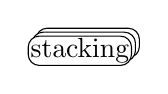
\begin{tikzpicture}[yscale=-1, baseline={(TEXT.base)}]
\node[draw, inner sep=0.3mm, fill=white, rounded corners, xshift=1mm, yshift=1mm] at (0,0)
{\phantom{stacking}};
\node[draw, inner sep=0.3mm, fill=white, rounded corners, xshift=0.5mm, yshift=0.5mm] at (0,0)
{\phantom{stacking}};
\node[draw, inner sep=0.3mm, fill=white, rounded corners] (TEXT) at (0,0) {stacking};
\end{tikzpicture}
effect to indicate a multiplicity of similar components.

The state of the system ($\var{SyState}$) comprises the state of each
device plus the contents of global memory, which is a partial function
from locations ($\var{Loc}$) to values ($\var{Val}$). We assume
that all values are mathematical integers, and that global memory
contains any location that is requested.

The state of a device ($\var{DvState}$) comprises the state of each of
its work-groups, the contents of the L2 cache, and a `lock file' that
records, for each location, whether it is locked in the L2 cache
($\padlock{d,w,t}$, where $d,w,t$ identifies the thread holding the
lock) or unlocked ($\unpadlock$). While a location is locked in the L2
cache by one thread, no other thread can read, write, evict, fetch, or
flush it.

The state of a work-group ($\var{WgState}$) comprises the state of
each of its threads, the contents of the L1 cache, plus an additional
lock that stalls the execution of RMW operations (and is taken by
threads executing remote RMW and store operations to ensure
atomicity). The state of a thread ($\var{ThState}$) comprises its
register file, which is a total function from registers to values. We
assume an unlimited number of registers.

A cache ($\var{Cache}$) comprises two components: a partial function
from locations to cache entries, and a synchronisation fifo. Each
entry ($\var{CacheEntry}$) comprises a value, a hygiene bit ($\CLEAN$
or $\DIRTY$), and a freshness bit ($\VALID$ or $\INVALID$). Note that
each location in memory has a separate cache entry
(cf.~Remark~\ref{rem:caching_protocols}). The synchronisation fifo
($\var{Fifo}$) is a hardware component introduced as part of AMD's
QuickRelease technology~\cite{hechtman+14}. It is a queue whose
elements ($\var{FifoEl}$) are locations that may need to be flushed to
the lower levels of the cache; by inserting flush markers
($\textsc{flush}$) among the locations, tagged with their own
device/work-group/thread identifier, threads can ascertain which
locations have been flushed. We assume that the $\mathrm{queue}$
datatype supports in-place $\mathrm{enqueue}()$ and
$\mathrm{dequeue}()$ methods, and exposes a $\mathrm{tail}$ field.

\begin{Notation} We write $\Sigma_{d}$ for
the state of device $d$, $\Sigma_{dw}$ for the state of work-group $w$
in that device, and $\Sigma_{dwt}$ for the state of thread $t$ in that
work-group. When we pass an $\var{Loc}$ $x$ to a $\var{Cache}$ $C$, writing $C(x)$, we are
implicitly looking up $x$ in the first of $C$'s two components.
\end{Notation}

\subsection{Assembly Language}
\label{sec:assembly_language}

\begin{table}
\centering
\setlength{\tabcolsep}{0.7mm}
\renewcommand\arraystretch{1.4}
\begin{tabular}{ll}
\hline
\rowcolor{black!20}
Instr. & \tstack{Effect on state $\Sigma$ when \\ executed by thread
$(d,w,t)$} \\
\hline
\cellcolor{black!10}\tstack{\INSld\,$r$\,$x$}
& \tstack{$\IF~\Sigma_{dw}.\mathrm{L1}(x).\mathrm{fr} =
\VALID~\THEN$ \\ 
\quad$\Sigma_{dwt}(r) :=
\Sigma_{dw}.\mathrm{L1}(x)$ \\ $\ELSE~\BLOCK$}
\\ 
\hline
\cellcolor{black!10}\tstack{\INSst\,$r$\,$x$}
& $\var{store}(\Sigma_{dw}.\mathrm{L1},x,\Sigma_{dwt}(r))$
\\ 
\hline
\cellcolor{black!10}\tstack{\INSincl1\,$r$\,$x$}
& \tstack{$\IF~\neg\var{ready}_{d,w,t}(\Sigma_{d\,w}.\mathrm{rmw})~\THEN~\BLOCK$ \\
$\ELSE~\IF~\Sigma_{dw}.\mathrm{L1}(x) = (v,\_,
\VALID)~\THEN$ \\ 
\quad$\Sigma_{dwt}(r) := v$ \\
\quad$\var{store}(\Sigma_{dw}.\mathrm{L1},x,v+1)$ \\
$\ELSE~\BLOCK$}
\\ 
\hline
\cellcolor{black!10}\tstack{\INSincl2\,$r$\,$x$}
& \tstack{$\IF~\neg\var{ready}_{d,w,t}(\Sigma_{d\,w}.\mathrm{rmw})~\THEN~\BLOCK$ \\ $\ELSE~\IF~\Sigma_{dw}.\mathrm{L1}(x).\mathrm{hy} =
\DIRTY~\THEN~\BLOCK$ \\
$\ELSE~\IF~\neg\var{ready}_{d,w,t}(\Sigma_{d}.\mathrm{lockfile}(x))~\THEN~\BLOCK$ \\
$\ELSE~\IF~\Sigma_{d}.\mathrm{L2}(x) =
(v,\_,\VALID)~\THEN$\\
\quad$\var{invalidate}(\Sigma_{dw}.\mathrm{L1},x)$ \\
\quad$\forall d'\ldotp
\var{invalidate}(\Sigma_{d'}.\mathrm{L2},x)$ \\
\quad$\Sigma_{dwt}(r) := v$ \\
\quad$\var{store}(\Sigma_{d}.\mathrm{L2},x,v+1)$ \\
$\ELSE~\BLOCK$}
\\ 
\hline
\cellcolor{black!10}\tstack{\INSflushl1\,\texttt{WG}}
& $\Sigma_{dw}. \mathrm{L1}.\mathrm{fifo}.\mathrm{enqueue}(\textsc{flush}_{d,w,t})$
\\ 
\hline
\cellcolor{black!10}\tstack{\INSflushl1\,\texttt{DV}}
& $\forall w'\ldotp \Sigma_{dw'}. \mathrm{L1}.\mathrm{fifo}.\mathrm{enqueue}(\textsc{flush}_{d,w,t})$
\\ 
\hline
\cellcolor{black!10}\tstack{\INSflushl1\,\texttt{SY}}
& $\forall d'\ldotp \forall w'\ldotp \Sigma_{d'w'}. \mathrm{L1}.\mathrm{fifo}.\mathrm{enqueue}(\textsc{flush}_{d,w,t})$
\\
\hline
\cellcolor{black!10}\tstack{\INSflushl2\,\texttt{DV}}
& $\Sigma_{d}. \mathrm{L2}.\mathrm{fifo}.\mathrm{enqueue}(\textsc{flush}_{d,w,t})$
\\ 
\hline
\cellcolor{black!10}\tstack{\INSflushl2\,\texttt{SY}}
& $\forall d'\ldotp \Sigma_{d'}. \mathrm{L2}.\mathrm{fifo}.\mathrm{enqueue}(\textsc{flush}_{d,w,t})$
\\ 
\hline
\cellcolor{black!10}\tstack{\INSinvall1\,\texttt{WG}}
& $\forall x\ldotp \var{invalidate}(\Sigma_{dw}. \mathrm{L1},x)$
\\ 
\hline
\cellcolor{black!10}\tstack{\INSinvall1\,\texttt{DV}}
& $\forall w'\ldotp\forall x\ldotp
\var{invalidate}(\Sigma_{dw'}. \mathrm{L1},x)$
\\ 
\hline
\cellcolor{black!10}\tstack{\INSinvall1\,\texttt{SY}}
& $\forall d'\ldotp \forall w'\ldotp \forall x
\ldotp \var{invalidate}(\Sigma_{d'w'}. \mathrm{L1},x)$
\\
\hline
\cellcolor{black!10}\tstack{\INSlk{L2}\,$x$}
& \tstack{$\IF~\neg\var{ready}_{d,w,t}(\Sigma_{d}.\mathrm{lockfile}(x))~\THEN~\BLOCK$ \\ $\ELSE~\Sigma_{d}.\mathrm{lockfile}(x) :=
\padlock{d,w,t}$}
\\
\hline
\cellcolor{black!10}\tstack{\INSul{L2}\,$x$}
& $\Sigma_{d}.\mathrm{lockfile}(x) := \unpadlock$
\\
\hline
\cellcolor{black!10}\tstack{\INSlk{rmw}\,\texttt{DV}}
& \tstack{$\IF~\exists w'\ldotp \neg\var{ready}_{d,w,t}(\Sigma_{d\,w'}.\mathrm{rmw})~\THEN~\BLOCK$ \\ $\ELSE~\forall w'\ldotp\Sigma_{d\,w'}.\mathrm{rmw} := \padlock{d,w,t}$}
\\
\hline
\cellcolor{black!10}\tstack{\INSlk{rmw}\,\texttt{SY}}
& \tstack{$\IF~\exists d'\ldotp\exists w'\ldotp \neg\var{ready}_{d,w,t}(\Sigma_{d'\,w'}.\mathrm{rmw})~\THEN~\BLOCK$ \\ $\ELSE~\forall d'\ldotp \forall w'\ldotp\Sigma_{d'\,w'}.\mathrm{rmw} := \padlock{d,w,t}$}
\\
\hline
\cellcolor{black!10}\tstack{\INSul{rmw}\,\texttt{DV}}
& $\forall w'\ldotp\Sigma_{d\,w'}.\mathrm{rmw} := \unpadlock$
\\
\hline
\cellcolor{black!10}\tstack{\INSul{rmw}\,\texttt{SY}}
& $\forall d'\ldotp \forall w'\ldotp\Sigma_{d'\,w'}.\mathrm{rmw} := \unpadlock$
\\
\hline
\end{tabular}
\par\vspace*{1mm}
\raggedright where:
\begin{eqnarray*}
\var{store}(C,x,v) &\eqdef& \stack{C(x) := (v,\DIRTY,\VALID)
\\ C.\mathrm{fifo}.\mathrm{enqueue}(x)} 
\\
\var{ready}_{d,w,t}(l) &\eqdef& (l = \padlock{d,w,t}) \vee (l =
\unpadlock)
\\
\var{invalidate}(C,x) &\eqdef& \stack{\IF\,C(x)\!\neq\!\bot\,\THEN~C(x).\mathrm{fr} :=
\INVALID{}\\{}\ELSE\,\NOP}
\end{eqnarray*}
\vspace*{-3mm}
\caption{Semantics of assembly instructions}
\label{tab:assembly_semantics}
\end{table}

We formalise our assembly language so that the behaviour of each 
thread in each work-group in each device is specified independently.
Accordingly, and in keeping with our formalisation of OpenCL
(\S\ref{sec:formalising_opencl}), an assembly program is a list (devices) of
lists (work-groups) of lists (threads) of lists (instructions of a thread) of assembly instructions.

The assembly language instructions are listed in the left-hand column
of Table~\ref{tab:assembly_semantics}. In summary, we have: loading
from a location to a register, storing from a register to a location,
atomically incrementing a location in the L1/L2 cache (this being the
simplest representative of the class of atomic RMW operations), inserting a $\textsc{flush}$ marker into one or more L1
or L2 caches, invalidating all entries in one or more L1 caches,
locking/unlocking a location in the L2 cache, and obtaining/releasing
all of the RMW locks in the current work-group/device/system. Other
standard instructions, and in particular control flow
instructions, would be required to provide a complete set; we limit
the presentation here to those that manipulate the memory system.

Table~\ref{tab:assembly_semantics} also defines the effect of each
assembly instruction when executed from state $\Sigma$ by thread $t$
in work-group $w$ in device $d$. Formally, each instruction is
modelled as a non-deterministic state transformer: a function from
$\var{SyState}$ to $\mathcal P(\var{SyState})$. A blocked instruction
returns the empty set, denoted $\BLOCK$. For the time being, no
instruction produces more than one final state,\footnote{While
conducting our soundness proof, we make use of an alternative
semantics that `disengages' the memory system, making loads completely
non-deterministic.} so we define each instruction using deterministic,
imperative pseudocode. We overload the $\forall$-operator to provide
an imperative \textbf{foreach} construct, leaving the bounds implicit.

These pieces of pseudocode leave only one other aspect of the
instructions' behaviours implicit: each piece of pseudocode, $\var{action}$, should be made conditional as follows:
\[
\IF~\var{unflushed}_{d, w, t}(\Sigma)~\THEN~\BLOCK~\ELSE~\var{action}
\]
where
\[
\stack{\var{unflushed}_{d, w, t}(\Sigma) \eqdef {}\\\qquad (\exists
d'\ldotp\textsc{flush}_{d,w,t}
\in\Sigma_{d'}.\mathrm{L2}.\mathrm{fifo}) \vee {}\\\qquad (\exists d',w'\ldotp \textsc{flush}_{d,w,t}
\in\Sigma_{d'w'}.\mathrm{L1}.\mathrm{fifo}).}
\]
That is, a thread that has placed a $\textsc{flush}$ marker in an L1 or L2 fifo must block until its marker is dequeued.

\paragraph{Loads and stores} 
Regarding loads (\INSld) from location $x$: if $x$'s L1 cache entry is
valid, the cached value is copied into the register file accordingly.
Otherwise, the instruction blocks, waiting for the environment to
fetch a valid entry from deeper in the cache hierarchy. In practice,
the load would initiate this fetch, but since our interest is in
checking safety properties, the existence of an environmental
transition that will fetch the new entry means that it suffices to
suppose that the load simply blocks.  We describe environmental transitions in \S\ref{sec:environmental_transitions}.

Stores (\INSst) to location $x$ simply write to $x$'s L1 entry, adding
a new entry if none exists, and overwriting any previous entry. The
entry is marked dirty and valid (via the $\var{store}$ helper
function) and the location is enqueued to the cache's synchronisation
fifo.

\paragraph{Atomic increments}
The \INSincl1 and \INSincl2 instructions are RMW operations, so they
block if the $\mathrm{rmw}$ lock is held by another thread. \INSincl1
increments $x$ in the L1 cache, writing the original value to the
given register; it blocks until the L1 cache holds a valid entry for
$x$ (as with loads, we rely on environmental transitions to provide
this valid entry). If the L1 entry for $x$ is dirty, the instruction
blocks until it is flushed; otherwise, the L1 entry, if present, is
invalidated. If access to $x$'s L2 entry is forbidden (by another
thread holding $x$'s $\mathrm{lockfile}$ entry), then the instruction
blocks. The instruction also blocks if $x$'s L2 entry is invalid or
absent; otherwise it increments $x$ in the L2 cache. When storing to
the L2 cache, all of $x$'s entries in other devices' L2 caches are
invalidated (via the
$\forall d'\ldotp \var{invalidate}(\Sigma_{d'}.\mathrm{L2},x)$ step), to
preserve cache coherence.

\paragraph{Flushes and invalidates}
The $\INSflushl1$ instruction enqueues a flush marker, tagged with the
current thread's identifier, into the current L1 cache, or all L1
caches in the current device, or all L1 caches in the system,
depending on whether the instruction is parameterised by \texttt{WG},
\texttt{DV}, or \texttt{SY}, respectively. $\INSflushl2$ enqueues a
flush marker into the current L2 cache, or all L2 caches in the
system, depending on whether it is parameterised by \texttt{DV} or
\texttt{SY}, respectively. The
$\INSinvall1\,\{\texttt{WG}, \texttt{DV}, \texttt{SY}\}$ instruction
invalidates all entries in all L1 caches in the $\{$work-group,
device, system$\}$.

\paragraph{Locks}
$\INSlk{L2}\,x$ and $\INSul{L2}\,x$ respectively lock and unlock the
location $x$ in the current L2 cache, the former blocking if the lock
is currently held by another thread. $\INSlk{rmw}$ and $\INSul{rmw}$
respectively obtain and release all the $\mathrm{rmw}$ locks in the
given scope. While a work-group's $\mathrm{rmw}$ lock is held by one
thread, no other thread in that work-group can perform an RMW
operation.

\paragraph{Reducing non-standard hardware requirements}
Some of the instructions above require non-standard hardware support:
specifically, the ability for a thread to flush/invalidate caches that
are not in its direct path to global memory, to lock cachelines, and
to lock RMW operations~\cite[\S4.4]{orr+15}. An attractive feature of
the revised RSP implementation inspired by our formalisation effort (\S\ref{sec:compilation_scheme}) is
that it does \emph{not} use cacheline locking, and thus requires less
non-standard hardware.


\subsection{Environmental Transitions}
\label{sec:environmental_transitions}

\begin{table}
\centering
\setlength{\tabcolsep}{1.0mm}
\renewcommand\arraystretch{1.5}
\begin{tabular}{ll}
\hline
\rowcolor{black!20}
Name & \tstack{Effect on state $\Sigma$ when \\ triggered by thread $(d,w,t)$} \\
\hline
\cellcolor{black!10}$\ACTevict1(x)$ & \tstack{$\IF~\Sigma_{dw}. \mathrm{L1}(x).\mathrm{hy} =
\CLEAN~\THEN$ \\ 
\quad$\Sigma_{dw}. \mathrm{L1}(x) := \bot$
} \\
\hline
\cellcolor{black!10}$\ACTevict2(x)$ & \tstack{$\IF~\Sigma_{d}. \mathrm{L2}(x).\mathrm{hy} =
\CLEAN$ \\ $\textbf{and}~\var{ready}_{d,w,t}(\Sigma_{d}.\mathrm{lockfile}(x))~\THEN$ \\
\quad$\Sigma_{d}. \mathrm{L2}(x) := \bot$} \\
\hline
\cellcolor{black!10}$\ACTflush1(x,v)$ & \tstack{$\IF~\Sigma_{dw}.\mathrm{L1}(x) = (v,
\DIRTY,\_)$\\ $\textbf{and}~\var{ready}_{d,w,t}(\Sigma_{d}.\mathrm{lockfile}(x))~\THEN$ \\ 
\quad$\forall d'\ldotp
\Sigma_{d'}.\mathrm{L2}(x).\mathrm{fr} := \INVALID$ \\
\quad$\var{store}(\Sigma_{d}.\mathrm{L2},x,v)$ \\
\quad$\Sigma_{dw}. \mathrm{L1}(x).\mathrm{hy} := \CLEAN$}\\
\hline
\cellcolor{black!10}$\ACTflush2(x,v)$ & \tstack{$\IF~\Sigma_{d}.\mathrm{L2}(x) = (v,
\DIRTY,\_)$\\ $\textbf{and}~\var{ready}_{d,w,t}(\Sigma_{d}.\mathrm{lockfile}(x))~\THEN$ \\ \quad$\Sigma.\mathrm{gl}(x) := v$ \\ \quad$\Sigma_{d}. \mathrm{L2}(x).\mathrm{hy} := \CLEAN$}\\
\hline
\cellcolor{black!10}$\ACTfetch1(x,v)$ &
\tstack{$\IF~\var{notDirty}(\Sigma_{dw}.\mathrm{L1},x)$\\ $\textbf{and}~\Sigma_{d}.\mathrm{L2}(x) = (v,\_,\VALID)$\\
$\textbf{and}~\var{ready}_{d,w,t}(\Sigma_{d}.\mathrm{lockfile}(x))~\THEN$\\\quad$\Sigma_{dw}.\mathrm{L1}(x) := (v,\CLEAN,\VALID)$}\\
\hline
\cellcolor{black!10}$\ACTfetch2(x,v)$ &
\tstack{$\IF~\var{notDirty}(\Sigma_{d}.\mathrm{L2},x)~\textbf{and}~\Sigma.\mathrm{gl}(x) = v$\\
$\textbf{and}~\var{ready}_{d,w,t}(\Sigma_{d}.\mathrm{lockfile}(x))~\THEN$ \\ \quad $\Sigma_{d}.\mathrm{L2}(x) := (v,\CLEAN,\VALID)$}\\
\hline
\cellcolor{black!10}$\ACTdeqaddr1(x)$ & \tstack{$\IF~\Sigma_{dw}.\mathrm{L1}.\mathrm{fifo}.\mathrm{tail} = x$ \\ $\textbf{and}~\var{notDirty}(\Sigma_{dw}.\mathrm{L1},x)~\THEN$ \\ \quad $\Sigma_{dw}.\mathrm{L1}.\mathrm{fifo}.\mathrm{dequeue}()$} \\
\hline
\cellcolor{black!10}$\ACTdeqaddr2(x)$ &
\tstack{$\IF~\Sigma_{d}.\mathrm{L2}.\mathrm{fifo}.\mathrm{tail} =
x$ \\ $\textbf{and}~\var{notDirty}(\Sigma_{d}.\mathrm{L2},x)~\THEN$ \\ \quad
$\Sigma_{d}.\mathrm{L2}.\mathrm{fifo}.\mathrm{dequeue}()$} \\
\hline
\cellcolor{black!10}$\ACTdeqmarker1$ & \tstack{$\IF~\Sigma_{dw}.\mathrm{L1}.\mathrm{fifo}.\mathrm{tail} =
\textsc{flush} ~\THEN$ \\ \quad $\Sigma_{dw}.\mathrm{L1}.\mathrm{fifo}.\mathrm{dequeue}()$} \\
\hline
\cellcolor{black!10}$\ACTdeqmarker2$ & \tstack{$\IF~\Sigma_{d}.\mathrm{L2}.\mathrm{fifo}.\mathrm{tail} =
\textsc{flush} ~\THEN$ \\ \quad $\Sigma_{d}.\mathrm{L2}.\mathrm{fifo}.\mathrm{dequeue}()$} \\
\hline
\end{tabular}
\par\medskip
\raggedright where:
\begin{eqnarray*}
\var{notDirty}(C,x) &\eqdef& (C(x) = \bot) \vee (C(x).\mathrm{hy}
= \CLEAN)
\end{eqnarray*}
\caption{Environmental transitions}
\label{tab:environmental_transitions}
\end{table}

At any time, the `environment' can transform the system
state. Environment transitions do not correspond to program
instructions, but each is triggered by a particular thread.

Locks aside, we point out that if an instruction is blocked, there is
always an environmental transition, or a series of environmental
transitions, that will result in the instruction becoming unblocked.
Locks, meanwhile, present the possibility of deadlock if used carelessly.

The available environmental transitions are defined, in
Tab.~\ref{tab:environmental_transitions}, by their effect on the
current system state $\Sigma$. Each cell in the right-hand column of
the table takes the form $\IF~\var{precondition}~\THEN~\var{action}$,
to reflect the fact that the transition can only occur under certain
conditions. 

The transitions are: evicting a clean cache entry (\ACTevict1 and
\ACTevict2), flushing a dirty cache entry and marking it clean
(\ACTflush1 and \ACTflush2), replacing a clean-or-absent cache
entry by fetching from the level below (\ACTfetch1 and \ACTfetch2),
removing a location whose cache entry is clean-or-absent from the tail
of a fifo (\ACTdeqaddr1 and \ACTdeqaddr2), and removing a
$\textsc{flush}$ marker from the tail of a fifo (\ACTdeqmarker1 and
\ACTdeqmarker2).

Regarding the $\ACTfetch1$ action, notice that the
newly-fetched entry is always marked \CLEAN, even if the L2 entry is
\DIRTY. There is no need to mark the L1 copy as dirty: the value
it holds is the same as the value that will be propagated to global
memory once the L2 entry (eventually) flushes.


\begin{Remark}[On caching protocols] 
\label{rem:caching_protocols}
%
We model caches as if each cacheline holds the contents of a single
location, but real cachelines hold the contents of several consecutive
locations. Therefore, real caches may fetch more than just the
requested location; we model this by allowing any location to be fetched
at any time. Real caches may flush multiple locations simultaneously,
but since they use a dirty bit mask, it is as if the flush is
per-location. Real cacheline locking may restrict access to more
locations than our model suggests, but this extra locking can only
lead to fewer behaviours, thus making our model sound. The caches used
in the evaluated design are \emph{write-through} and
\emph{write-allocate}~\cite[Tab.~1]{orr+15};\footnote{The original RSP description reported the caches as being \emph{write-no-allocate}, but we
confirm that this was in error.} we safely capture
write-through behaviour by allowing the environment to flush at any
time, and write-allocate behaviour by having \INSst{} create a cache
entry if none exists.
%
\end{Remark}

\subsection{Compilation Scheme}
\label{sec:compilation_scheme}

We now consider the compilation of OpenCL+RSP programs into the
assembly language of \S\ref{sec:assembly_language}. 

Although our assembly language can apply to a multiple-device system,
this subsection, in line with the original RSP proposal, considers
only the single-device case~\cite[\S5]{orr+15}. This means that our
compilation scheme does not extend to OpenCL+RSP operations that use $\sall$-scope.

The compilation scheme shown in the `Original' column of
Tab.~\ref{tab:compilation_scheme} is what we believe to be a faithful
representation of the original proposed scheme~\cite{orr+15}, informed by a series of interviews with
the broader set of RSP designers. As a result of our formalisation work, we
have found problems with this scheme, which we elucidate in
\S\ref{sec:problems_compilation_scheme}. We propose instead the
compilation scheme shown in the `Proposed' column of
Tab.~\ref{tab:compilation_scheme}, which addresses these problems.  We
now explain and justify our proposed scheme; a proof that it is sound
follows in \S\ref{sec:soundness}.

Our explanation centres on how the compilation scheme ensures correct
release/acquire semantics (so that inter-work-group message-passing programs, such as
\[
\begin{array}{l|||l}
\texttt{store}_{\na}(\texttt{x}, 42)\texttt{;} &
\texttt{if}(\texttt{r0} = \texttt{load}_{\sdv,\texttt{N}}(\texttt{y}))\\
\texttt{store}_{\sdv, \texttt{N}}(\texttt{y}, 1)\texttt{;} &
\texttt{~r1} = \texttt{load}_{\na}(\texttt{x})\texttt{;}
\end{array}
\]
can never yield $\{\texttt{r0}=1, \texttt{r1}=0\}$) and also ensures
RMW atomicity (so that programs
like the one in Example~\ref{ex:rmw_atomicity_3} can never finish with $\texttt{x}=1$).


\begin{table}[t]
\centering
\setlength{\tabcolsep}{2mm}
\renewcommand\arraystretch{1.5}
\begin{tabular}{llll}
\hline
\rowcolor{black!20} 
\multicolumn{2}{l}{OpenCL+RSP operation} & Original & Proposed
\\ \hline
\cellcolor{black!10}\ding{182} & 
\cellcolor{black!10}\tmstack{$r = \texttt{load}_{\na}(x)$
\\ $r = \texttt{load}_{\swg, \_}(x)$}& 
$\INSld\,r\,x$ &
$\INSld\,r\,x$
\\ \hline
\cellcolor{black!10}\ding{183} & 
\cellcolor{black!10}\tstack{$r = \texttt{load}_{\sdv,\texttt{N}}(x)$} & 
\tstack{
$\INSinvall1\,\texttt{WG}$ \\ 
$\INSld\,r\,x$} & 
\tstack{
$\INSld\,r\,x$ \\ 
$\INSinvall1\,\texttt{WG}$}
\\ \hline
\cellcolor{black!10}\ding{184} & 
\cellcolor{black!10}\tstack{$r = \texttt{load}_{\sdv, \texttt{R}}(x)$}&
\tstack{
$\INSlk{L2}\,x$ \\ 
~~$\INSflushl1\,\texttt{DV}$ \\ 
~~$\INSinvall1\,\texttt{WG}$ \\
~~$\INSld\,r\,x$ \\ 
$\INSul{L2}\,x$} 
&
\tstack{
$\INSld\,r\,x$ \\ 
$\INSflushl1\,\texttt{DV}$ \\ 
$\INSinvall1\,\texttt{WG}$}
\\ \hline
\cellcolor{black!10}\ding{185} & 
\cellcolor{black!10}\tmstack{$\texttt{store}_{\na}(x, r)$\\$\texttt{store}_{\swg, \_}(x, r)$} & 
$\INSst\,r\,x$ & 
$\INSst\,r\,x$
\\ \hline
\cellcolor{black!10}\ding{186} & 
\cellcolor{black!10}\tstack{$\texttt{store}_{\sdv, \texttt{N}}(x, r)$} & 
\tstack{
$\INSflushl1\,\texttt{WG}$ \\ 
$\INSst\,r\,x$} 
& 
\tstack{
$\INSflushl1\,\texttt{WG}$ \\ 
$\INSst\,r\,x$} 
\\ \hline
\cellcolor{black!10}\ding{187} & 
\cellcolor{black!10}\tstack{$\texttt{store}_{\sdv, \texttt{R}}(x, r)$} 
& 
\tstack{
$\INSlk{L2}\,x$ \\ 
~~$\INSflushl1\,\texttt{WG}$ \\ 
~~$\INSst\,r\,x$ \\ 
~~$\INSinvall1\,\sdv$ \\ 
$\INSul{L2}\,x$} & 
\tstack{
$\INSlk{rmw}\,\texttt{DV}$ \\
~~$\INSflushl1\,\sdv$ \\ 
~~$\INSinvall1\,\sdv$ \\ 
~~$\INSst\,r\,x$ \\
~~$\INSflushl1\,\swg$ \\ 
~~$\INSinvall1\,\sdv$ \\ 
$\INSul{rmw}\,\texttt{DV}$}
\\ \hline
\cellcolor{black!10}\ding{188} & 
\cellcolor{black!10}\tstack{$r = \texttt{fetch\_inc}_{\swg, \_}(x)$} & 
\tstack{$\INSincl1\,r\,x$} &
\tstack{$\INSincl1\,r\,x$}
\\ \hline
\cellcolor{black!10}\ding{189} & 
\cellcolor{black!10}\tstack{$r = \texttt{fetch\_inc}_{\sdv, \texttt{N}}(x)$} & 
\tstack{$\INSflushl1\,\texttt{WG}$ \\ 
$\INSinvall1\,\texttt{WG}$ \\
$\INSincl2\,r\,x$} &
\tstack{$\INSflushl1\,\texttt{WG}$ \\
$\INSincl2\,r\,x$ \\
$\INSinvall1\,\texttt{WG}$}
\\ \hline
\cellcolor{black!10}\ding{190} & 
\cellcolor{black!10}\tstack{$r = \texttt{fetch\_inc}_{\sdv, \texttt{R}}(x)$} & 
\tstack{$\INSlk{rmw}\,\texttt{DV}$ \\
~~$\INSlk{L2}\,x$ \\ 
~~~~$\INSflushl1\,\texttt{DV}$ \\ 
~~~~$\INSinvall1\,\texttt{WG}$ \\
~~~~$\INSincl2\,r\,x$ \\ 
~~~~$\INSinvall1\,\texttt{DV}$ \\
~~$\INSul{L2}\,x$ \\
$\INSul{rmw}\,\texttt{DV}$ } 
&
\tstack{
$\INSlk{rmw}\,\texttt{DV}$ \\
~~$\INSflushl1\,\texttt{DV}$ \\
~~$\INSinvall1\,\texttt{DV}$ \\
~~$\INSincl2\,r\,x$ \\
~~$\INSflushl1\,\texttt{DV}$ \\
~~$\INSinvall1\,\texttt{DV}$ \\
$\INSul{rmw}\,\texttt{DV}$}
\\
\hline 
\end{tabular}
\caption{Compilation schemes, original and proposed}
\label{tab:compilation_scheme}
\end{table}

\paragraph{Loads}
An OpenCL load that is non-atomic ($\na$) or at work-group ($\swg$) scope is
compiled to a lone \INSld{} instruction~\ding{182}. No further
instructions are required because consistency need only be enforced as
far as the L1 cache, which \INSld{} already targets natively. For a
load at $\sdv$ scope~\ding{183}, we ensure `acquire' semantics by
invalidating the L1 cache after the \INSld{}. This ensures that
subsequent loads observe values from the L2 cache.

To upgrade the load to a remote load, the invalidation is preceded by
a flush of all the L1 caches in the device~\ding{184}; this ensures
that subsequent loads observe values that have been written to any L1
cache.

\paragraph{Stores}
As for loads, non-atomic or $\wg$-scope stores
are compiled to lone \INSst{} instructions~\ding{185}. For a store at
$\sdv$ scope, we ensure `release' semantics by flushing the L1 cache before the \INSst{}. This
ensure that prior stores are visible to operations that subsequently
read from the L2 cache~\ding{186}. 

To upgrade to a remote store~\ding{187}, we must also ensure that
prior stores are visible to operations that subsequently read from
their own L1 cache. For this, we precede the $\INSst$ instruction with
a remote invalidate ($\INSinvall1\,\sdv$). The other instructions are
present to ensure that any $\wg$-scoped increments, simultaneously
executing on different work-group, are performed atomically. Without
them, we might observe such violations of RMW atomicity as were seen
earlier in Example~\ref{ex:rmw_atomicity_2}. Naturally, these
increments cannot happen between the $\INSlk{rmw}$ and $\INSul{rmw}$
instructions. In case one happens \emph{before} the $\INSlk{rmw}$, we
use a remote flush ($\INSflushl1\,\sdv$) to ensure that it is promptly
flushed, and thus unable to overwrite our upcoming store. In case one
happens \emph{after} the $\INSul{rmw}$, we use a local flush and a
remote invalidate after our store, to ensure that the increment will
observe our stored value.

\paragraph{Atomic increments}
We map the atomic fetch-and-increment operation, \texttt{fetch\_inc},
to the \texttt{INC} assembly instruction. At $\swg$ scope, the \texttt{INC} operation acts on the L1
cache~\ding{188}, and at $\sdv$ scope, it acts directly on the L2
cache~\ding{189}. Performing the operation directly on the L2 cache
(rather than on the L1 cache and then flushing) ensures the atomicity
of RMW operations. Moreover, at $\sdv$ scope, the \texttt{fetch\_inc}
must provide acquire+release semantics. Accordingly, it begins with a
flush (inherited from the release store,~\ding{186}) and finishes with
an invalidate (inherited from the acquire load,~\ding{183}).

Upgrading to a remote increment imposes several
requirements~\ding{190}. To ensure acquire semantics, the remote
increment must end with (at least) a remote-flush and a
local-invalidate (as for the remote load discussed above). To ensure
release semantics, it must begin with (at least) a local-flush and a
remote-invalidate (as for the remote store). For RMW atomicity, it
must observe any concurrent increments on another L1 cache that occur
before the RMW lock is acquired, and any that happen after the RMW
lock is released must observe the newly-incremented value. Therefore,
the remote increment must begin with (at least) a remote-flush and a
local-invalidate, and end with (at least) a local-flush and a
remote-invalidate. Merging all these constraints together, we find
remote flushes and invalidates are required both before and after the
$\INSincl2$.

\subsection{Problems with the Original Scheme}
\label{sec:problems_compilation_scheme}

We describe two errors in the original compilation
scheme (Tab.~\ref{tab:compilation_scheme}, `Original' column), and
explain how our proposed scheme (`Proposed' column) addresses
them. Finding these issues early in the design process is, we
believe, the key value of formalisation efforts such as ours.

\begin{figure}
\renewcommand\tabcolsep{0.5mm}
\centering
\begin{tabular}{l|c|l}
\textbf{Thread 1} (executing & \textbf{L2 cache} & \textbf{Thread 2}
(executing \\
{$\texttt{store}_{\na}(\texttt{x},42)\texttt{;}$} & &
{$\texttt{if}(\texttt{r0}=\texttt{load}_{\sdv,\texttt{N}}(\texttt{y}))$} \\
{$\texttt{store}_{\sdv,\texttt{N}}(\texttt{y},1)\texttt{;}$} ) & & {$\texttt{~r1}=\texttt{load}_{\na}(\texttt{x})\texttt{;}$} ) \\
\hline
\lonestate{\,} & \ltwostate{\ltwoce{\texttt{x}}{0}\\\ltwoce{\texttt{y}}{0}} & \lonestate{\,} \\
& & $\INSinvall1\,\swg$ \\
& & \lonestate{\,} \\
& & \env{$\ACTfetch1(\texttt{x},0)$} \\
& & \lonestate{\loneceCV{\texttt{x}}{0}} \\
$\INSst\,42\,\texttt{x}$ & & \\
\lonestate[\texttt{x}]{\loneceDV{\texttt{x}}{42}} & & \\
\env{$\ACTflush1(\texttt{x},42)$} & & \\
\lonestate[\texttt{x}]{\loneceCV{\texttt{x}}{42}}
& \ltwostate{\ltwoce{\texttt{x}}{42}\\\ltwoce{\texttt{y}}{0}} & \\
$\INSflushl1\,\swg$ & & \\
\lonestate[\textsc{flush}\\\texttt{x}]{\loneceCV{\texttt{x}}{42}}
& & \\
\env{$\ACTdeqaddr1$} & & \\
\lonestate[\textsc{flush}]{\loneceCV{\texttt{x}}{42}} & & \\
\env{$\ACTdeqmarker1$} & & \\
\lonestate{\loneceCV{\texttt{x}}{42}} & & \\
$\INSst\,1\,\texttt{y}$ & & \\
\lonestate[\texttt{y}]{\loneceCV{\texttt{x}}{42}\\\loneceDV{\texttt{y}}{1}} & & \\
\env{$\ACTflush1(\texttt{y},1)$} & & \\
\lonestate[\texttt{y}]{\loneceCV{\texttt{x}}{42}\\\loneceCV{\texttt{y}}{1}}
& \ltwostate{\ltwoce{\texttt{x}}{42}\\\ltwoce{\texttt{y}}{1}} & \\
& & \env{$\ACTfetch1(\texttt{y},1)$} \\
& & \lonestate{\loneceCV{\texttt{x}}{0}\\\loneceCV{\texttt{y}}{1}} \\
& & $\INSld\,\texttt{r0}\,\texttt{y}$ \\
& & $\INSld\,\texttt{r1}\,\texttt{x}$ \\
\end{tabular} 

\caption{An execution of inter-work-group message-passing that leads
to the illegal final state $\{\texttt{r0}=1,\texttt{r1}=0\}$}
\label{fig:mp_violation}
\end{figure}

\subsubsection{Non-Remote Loads Can Violate Message-Passing}
Because $\sdv$-scoped non-remote loads (\ding{183} in
Tab.~\ref{tab:compilation_scheme}) invalidate their L1 cache
\emph{before} the \INSld{}~\cite[\S2.3]{orr+15}, coherence (axiom
\axiom{Coh} in Fig.~\ref{fig:openclmm}) is violated. To explain this,
Fig.~\ref{fig:mp_violation} exhibits a machine execution, obtained by
compiling a basic inter-work-group message-passing idiom, that leads
to a prohibited final state. The vertical order in the figure
illustrates the interleaving of each thread's instructions and
environment transitions, and we include frequent snapshots of the
machine's state. In braces, we show the cache entries (using
$\textsc{c}=\textsc{clean}$, $\textsc{d}=\textsc{dirty}$,
$\textsc{v}=\textsc{valid}$, and $\textsc{i}=\textsc{invalid}$), and
in brackets we show the contents of non-empty synchronisation
fifos. Since our compilation scheme covers only the single device
case, we treat the shared L2 cache as if it is global memory.

Initially, all memory is zeroed and all caches are empty. If
\texttt{r0} observes $1$, then coherence on \texttt{x} dictates that
\texttt{r1} must observe $42$. Thread 2 invalidates its L1 cache, but
then the environment immediately repopulates it with \texttt{x}'s
initial value. Thread 1 (which, being in a different work-group, has
its own L1 cache) then stores new values for \texttt{x} and \texttt{y}
into the L2 cache. When Thread 2 resumes, it fetches the updated
\texttt{y}, but reads the stale \texttt{x} from its own L1 cache.

This bug recurs
in non-remote $\sdv$-scoped increments (\ding{189} in
Tab.~\ref{tab:compilation_scheme}): the invalidate preceding the
\INSincl2{} instruction leads to a similar message-passing violation.

The inversion of the \INSinvall1 and \INSld{} instructions is also
carried through to remote loads
(\ding{184})~\cite[\S4.2]{orr+15}. However, an undocumented detail of
the original implementation actually prevents the bug recurring in
this case. Specifically, accesses to the relevant L2 cacheline during
remote loads are stalled using \INSlk{L2} and \INSul{L2}
instructions. The problematic execution depicted in
Fig.~\ref{fig:mp_violation} relies on Thread 2 fetching \texttt{x}
after its L1 invalidation and before Thread 1 flushes its new
\texttt{x}. Cacheline locking prevents this from happening, and thus
restores coherence; however, it could lead to unnecessary inter-thread
interference, and is more complicated to reason about than our
proposed lock-free version.

\textbf{\itshape Our proposed scheme} avoids these problems by
invalidating the L1 cache \emph{after} performing the \INSld{}
instruction (\ding{183}) or the \INSincl2{} instruction (\ding{189}).
In the context of Fig.~\ref{fig:mp_violation}, this ensures that
\texttt{x} is re-fetched after loading \texttt{y}.

\begin{figure}
\renewcommand\tabcolsep{1mm}
\centering
\begin{tabular}{l|c|l}
\textbf{Thread 1} (executing & \textbf{L2 cache} & \textbf{Thread 2}
(executing \\ 
$\texttt{fetch\_inc}_{\swg,\texttt{N}}(\texttt{x})\texttt{;}$) & & $\texttt{store}_{\sdv,\texttt{R}}(\texttt{x},2)\texttt{;}$) \\
\hline
& \ltwostate{\ltwoce{\texttt{x}}{0}}
& \\
& & \env{$\ACTfetch1(\texttt{x},0)$} \\
& & \lonestate{\loneceCV{\texttt{x}}{0}} \\
\env{$\ACTfetch1(\texttt{x},0)$} & & \\
\lonestate{\loneceCV{\texttt{x}}{0}}
& & \\
$\INSincl1\,\texttt{x}$ & & \\
\lonestate[\texttt{x}]{\loneceDV{\texttt{x}}{1}}
& & \\
& & $\INSlk{L2}\,\texttt{x}$ \\
& & $\INSflushl1\,\swg$ \\
& &
\lonestate[\textsc{flush}]{\loneceCV{\texttt{x}}{0}} \\
& & \env{$\ACTdeqmarker1$} \\
& & \lonestate{\loneceCV{\texttt{x}}{0}} \\
& & $\INSst\,2\,\texttt{x}$ \\
& & \lonestate[\texttt{x}]{\loneceDV{\texttt{x}}{2}} \\
& & $\INSinvall1\,\sdv$ \\
\lonestate[\texttt{x}]{\loneceDI{\texttt{x}}{1}} 
& & \lonestate[\texttt{x}]{\loneceDI{\texttt{x}}{2}} \\
& & $\INSul{L2}\,\texttt{x}$ \\
& & \env{$\ACTflush1(\texttt{x},2)$} \\
& \ltwostate{\ltwoce{\texttt{x}}{2}} & \lonestate[\texttt{x}]{\loneceCI{\texttt{x}}{2}} \\
\env{$\ACTflush1(\texttt{x},1)$} & & \\
\lonestate[\texttt{x}]{\loneceCI{\texttt{x}}{1}}
& \ltwostate{\ltwoce{\texttt{x}}{1}} & \\
\end{tabular} 
\caption{An execution of the program in
Example~\ref{ex:rmw_atomicity_3} that leads to the illegal
final state $\{\texttt{x}=1\}$}
\label{fig:rmw_violation}
\end{figure}

\subsubsection{Remote Stores Can Violate RMW Atomicity}
The original implementation of $\sdv$-scoped remote stores (\ding{187}
in Tab.~\ref{tab:compilation_scheme}) does not ensure RMW atomicity
(axiom \axiom{Rmw} in Fig.~\ref{fig:openclmm}) in the presence of a
$\swg$-scoped increment in a different
work-group. Figure~\ref{fig:rmw_violation} exhibits an execution,
obtained by compiling the program in Example~\ref{ex:rmw_atomicity_3},
that leads to a prohibited final state.

Both threads begin by fetching $\texttt{x}=0$ into their L1
caches. Thread 1 performs its increment, which leaves its L1
cache holding $\texttt{x}=1$, then thread 2 writes $\texttt{x}=2$ into
its own L1 cache. Thread 2's write is flushed to the shared L2 first,
and then overwritten by Thread 1's write, to leave the final state of
$\texttt{x}=1$.

Thus the remote store does not force
local increments in other work-groups to flush their results to the
shared L2.

\textbf{\itshape Our proposed scheme} rectifies this by including a
$\sdv$-scoped flush (before the $\INSst$ instruction). This alone does
not restore RMW atomicity because a similar problem arises if Thread 1
fetches $\texttt{x}=0$ from the L2 cache after Thread 2 has released
its lock on \texttt{x}'s L2 cacheline but before it flushes
$\texttt{x}=2$. To deal with this situation, we include a further
flush (this time at $\swg$-scope) \emph{after} the $\INSst$
instruction.


\section{Proving Soundness}
\label{sec:soundness}

We now prove our remedied implementation of RSP
(Tab.~\ref{tab:compilation_scheme}, right column) to be sound. The existence of
this proof, which links the high-level OpenCL+RSP memory model
(\S\ref{sec:formalising_opencl+rsp}) to the low-level implementation
of OpenCL+RSP, lends assurance that the analysis we
performed on the litmus tests and work-stealing queue in
\S\ref{sec:testing} is not vacuous.

\subsection{Soundness Statement} 

The soundness theorem relates three components: the formal semantics
of the OpenCL+RSP language, the formal semantics of the assembly
language, and the compilation scheme for mapping programs for the
former to the latter. It essentially states that if $Q$ is the
assembly program that results from compiling an OpenCL+RSP program
$P$, then every execution of $Q$ is observationally equivalent to some
consistent execution of $P$.
%
The precise statement is as follows.

\begin{theorem}[Soundness] 
\label{thm:soundness}
For an OpenCL+RSP program $P$:
\[
\forall Y \in \Lsem{\var{compile}\,P}\ldotp \exists X \in
\Hsem{P}\ldotp X \cong Y 
\]
where $\Lsem{-}$ returns the set of executions of a given assembly
program, $\var{compile}$ applies the
mapping in Tab.~\ref{tab:compilation_scheme} (right column), $\Hsem{-}$ returns the set of executions allowed of a given OpenCL+RSP
program, and
$\cong$ captures a notion of observational equivalence between
executions. 
\end{theorem}

\paragraph{OpenCL+RSP executions}
Recall from
\S\ref{lab:candidate} that the pre-executions of an OpenCL+RSP program are those that can be
obtained under the assumption of a completely non-deterministic memory
(i.e., loads can obtain any value).  We write $\Hcand{-}$ for the set of candidate executions whose
pre-executions match a given OpenCL+RSP program.
%
The set of executions allowed of a given OpenCL+RSP program $P$,
written $\Hsem{P}$, is defined as either the set of consistent executions
(when none of them has a race) or the universal set (otherwise); that
is,
\[
\Hsem{P} \eqdef \begin{cases} \unv & \text{if $\exists X \in \var{Xs}\ldotp
\var{faulty}(X)$} \\ \var{Xs} & \text{otherwise} \end{cases}
\]
where $\var{Xs} \eqdef \{X \in \Hcand{P} \mid \var{consistent}(X)\}$.

\paragraph{Assembly executions} The set of executions allowed of a
given assembly program $Q$, written $\Lsem{Q}$, is the set of
all possible complete executions of the program under the
semantics of assembly instructions defined in
\S\ref{sec:assembly_language}. 
%
Given an initial state, each of an assembly program's completed executions
% possible final states
can be obtained by interleaving program actions
(Tab.~\ref{tab:assembly_semantics}) and environmental actions
(Tab.~\ref{tab:environmental_transitions}) until all of the program's
instructions have been dispatched (respecting the order in each
thread) and all of the caches have been flushed down to global memory.
%
Then, from each of these completed executions, we can project an
execution graph comprising the memory accesses that were made.
% the order in which writes occurred (the analogue of modification
% order), and for each read, the write whose value is read.
It is the set of these projected execution graphs that are
calculated by $\Lsem{-}$.

In fact, we implement the projection by augmenting the semantics of
instructions so as to transform not only the current state, but also
to accumulate the execution graph. This execution graph is initially
empty, and is extended with an additional event at each
program step. For instance, \INSld{} appends an $\mathrm{R}$ event,
while \INSincl1 appends an $\mathrm{RMW}$ event. Ultimately,
$\Lsem{-}$ is defined as the set of execution graphs that accompany
terminal states.

\paragraph{Assembly events}
Recall the OpenCL memory events defined in Fig.~\ref{fig:openclmm}:
\begin{equation}
\label{eq:opencl_events}
\mstack{\evWna(x,v) \mid \evRna(x,v) {}\\{} \mid \evW_s(x,v) \mid \evR_s(x,v) \mid \evRMW_s(x,v,v').}
\end{equation}
The events in an assembly execution are broadly similar to the OpenCL events, except that they omit the scope parameter $s$ (since the abstraction of
scopes does not exist at the assembly level) and include additional
events to represent low-level memory events that are not exposed
in OpenCL:
\begin{equation}
\label{eq:asm_events}
\mstack{\mathrm{W}(x,v) \mid \mathrm{R}(x,v) \mid \mathrm{RMW}(x,v,v')
{}\\{} \mid
\mathrm{FlushL1}_{\{\swg,\sdv\}} \mid
\mathrm{InvalL1}_{\{\swg,\sdv\}} {}\\{} \mid \mathrm{LockRMW}_{\{\swg,\sdv\}}
\mid \mathrm{UnlockRMW}_{\{\swg,\sdv\}}.}
\end{equation}
Since our proposed compilation scheme does away with cacheline
locking, we need not include events to represent $\INSlk{L2}$ and
$\INSul{L2}$ instructions.

\paragraph{Execution equivalence}
The $\cong$-relation of Thm.~\ref{thm:soundness} captures a notion of
equivalence between an OpenCL execution and an assembly execution.
Simply put, $X\cong Y$ holds if $X$ and $Y$ are isomorphic graphs once
the features that are specific to high-level or low-level executions -- scope parameters and low-level memory events --
are erased. We effectively reduce both $X$ and $Y$ to executions
whose event labels are restricted to the common sub-language of
\eqref{eq:opencl_events} and \eqref{eq:asm_events}:
\[
\mathrm{W}(x,v) \mid \mathrm{R}(x,v) \mid \mathrm{RMW}(x,v,v').
\]

\subsection{Structure of the Proof}

For a given program, the axiomatic OpenCL memory model acts on a set
of pre-executions, $\Hcand{P}$, computed by a thread-local counterpart
to the semantics. A faithful model of OpenCL's thread-local semantics
would be an extensive work in itself, and is beyond the scope of this
paper. Instead, we follow Batty~\cite{battythesis} and simply require
our thread-local semantics to only generate sets, $\Hcand{P}$, that
exhibit \emph{receptiveness}; given a pre-execution in $\Hcand{P}$
with a read event $r$, for every value $v$, there is another
pre-execution in $\Hcand{P}$ where all $(\rf \cup \Sb)^+$ predecessors
of $r$ are identical, but $r$ reads the value $v$, and the rest of the
execution may differ. This requirement is integral to the calculation
of the semantics: if the candidates in $\Hcand{P}$ do not cover the
range of values that might be read, then executions will be missed by
the memory model. To complement this, we prove \emph{completion}: that
any consistent $\rf \cup \Sb$ down-closed prefix of a pre-execution in
$\Hcand{P}$ can be completed to a consistent execution of $\Hsem{P}$.

The theorem describes the behaviour of programs, but because we are
working with an axiomatic memory model, the proof is most
conveniently performed at the level of executions. As a consequence,
we must lower some concepts to the level of executions, in particular
the compilation mapping and the notion of consistency for assembly
executions.  We write $\var{comp}\,X\,Y$ when the assembly execution
$Y$ is a valid compilation of the OpenCL execution $X$, according to
the mapping in Tab.~\ref{tab:compilation_scheme} (right column).  We
write $\var{consistent_\mathcal{A}}$ when the assembly execution $Y$
is permitted by the machine.

Now we present a soundness lemma over executions:

\begin{lemma}[Execution soundness] 
\label{lem:execution_soundness}
For all OpenCL+RSP programs $P$:
\[ 
\stack{\forall X_{\var{pre}} \in \Hcand{P}\ldotp 
\forall Y\ldotp \var{comp}\,X_{\var{pre}}\,Y \wedge
\var{consistent_\mathcal{A}}\,Y \implies {} \\ \qquad
\exists X\ldotp (\var{pre}\,X = X_{\var{pre}}) \wedge X \in \Hsem{P} \wedge X \cong Y}
\]
where $\var{\var{pre}}$ projects the
pre-execution from a candidate execution, removing $\mo$ and $\rf$.
\end{lemma}



We use this theorem to establish the program-level soundness theorem (Thm.~\ref{thm:soundness})
by constructing a $Y$ that satisfies $\var{comp}$ and
$\var{consistent_\mathcal{A}}$ in such a way that the set of
consistent executions of the compiled program,
$\Lsem{\var{compile}\,P}$, is equal to the set of consistent assembly
executions that $\var{comp}$ matches with the pre-executions of the
program.

In establishing execution soundness, we must be able to
prove that a given OpenCL pre-execution can be extended to a
consistent execution. To do so, we must find a modification order
($\var{mo}$) and a reads-from relation ($\var{rf}$) that together
satisfy the various consistency axioms. To this end, we further
augment the semantics of assembly programs so that they construct
witnesses for these relations as they execute.

\paragraph{Auxiliary state}
We augment machine states with two extra components. We emphasise that
these components are auxiliary (sometimes called `ghost'): they do not
affect the operation of the machine, existing only to accumulate
useful information for the proof.

We modify the types of cache entries and global memory so as to
accompany each value with both an event identifier and a list of event
identifiers. That is:
\[
\small
\renewcommand\arraystretch{1.3}
\begin{array}{@{}r@{~}c@{~}l@{}}
\var{Aux} &=& (\mathrm{rfsource}{:}\,\var{EventId}) \times (\mathrm{pmo}{:}\,\var{EventId}\,\mathrm{list}) \\
\var{CacheEntry} &=& \stack{\var{Val} \times \mhl{\var{Aux}} \times 
(\mathrm{hy}{:}\,\var{Hygiene}) \times
(\mathrm{fr}{:}\,\var{Freshness})} \\
\var{Global} &=& \var{Loc} \rightharpoonup (\var{Val} \times\mhl{\var{Aux}}).
\end{array}
\]
%
The new $\mathrm{rfsource}$ component identifies the event responsible
for writing the currently-held value. Whenever a location is written
to or flushed, this component is overwritten appropriately. If the
location is subsequently loaded, an $\var{rf}$-edge is drawn from this
event to the loading event.

The new $\mathrm{pmo}$ component (for `partial modification order')
identifies the sequence of events that have written to this cache entry
since it was last flushed. In the case of global memory, which is
never flushed, this component records a history of all the events that
have ever written to this location. Whenever a cache entry is fetched,
the newly fetched entry has its $\mathrm{pmo}$ component
initialised to the empty list. Whenever an entry is flushed, the
contents of its $\mathrm{pmo}$ list is appended to the end of the
$\mathrm{pmo}$ list in the deeper cache entry or global memory location,
and its $\mathrm{pmo}$ list is then cleared. When an assembly program
completes its execution and all the caches have been flushed down to
global memory, then a witness for the $\var{mo}$ relation can be read
off by taking the union of all the $\mathrm{pmo}$ components in global
memory.




\paragraph{Consistency}
It remains to show either that the pre-execution, combined with the
$\mo$ and $\rf$ relations generated by the abstract machine, is
consistent, or that the program was faulty, in which case every
execution is a member of $\Hsem{P}$.

If the program is racy, then the $\mo$ and $\rf$ relations may be
inconsistent, and these executions must be treated
differently. Consequently, we split the proof into two cases. In one
case, every $\rf$ edge on a non-atomic location is coincident with an
$\hb$ edge, and there are no increment accesses that race with badly
scoped writes. In the other case, there is
at least one $\rf$ edge that is not coincident with a read, or there
is a write that races with an increment that follows it in $\mo$.

We prove the first case, omitting the assumption that $X_{\var{pre}}$
is a pre-execution of the program $P$, and then rely on this in the
proof of the second.

\paragraph{Case 1: $\hb$ covers non-atomic $\rf$}
Five consistency axioms must be established (Fig.~\ref{fig:openclmm}): $\axiom{Hb}$,
$\axiom{Coh}$, $\axiom{Rf}$, $\axiom{Narf}$, and
$\axiom{Rmw}$.
%
For each axiom, we relate the forbidden shape to an assembly
execution, and consider the sequences of operations that the abstract
machine might perform to generate that execution. We collect
intermediate lemmas that relate the OpenCL+RSP candidate execution to
the states of the abstract machine.

More precisely, we build a machine execution version of the
happens-before relation, and we show that events related by $\hb$ at
the language level correspond to machine-execution events related by
the new relation. We then establish that when a write or a read
precedes an access of the same location in machine happens-before,
then this write, or the write that is read, in the case of a read, is
sure to have propagated through the memory hierarchy of the
other thread prior to its access. We use this property to establish
the axioms of the language model.

Take for example the axiom $\axiom{Rf}$. To prove this, we
establish that given an $\rf$ edge from a write, $w$, to a read, $r$,
the write must have propagated to the reading thread prior to the
read, and then, because of the $\hb$ edge, the write must also have
propagated to the writing thread before the write, a contradiction.
Then the cycle forbidden by $\axiom{Rf}$ is in fact forbidden
by the compilation scheme over the abstract machine.

This part of the proof is reminiscent of a previous
compilation-scheme proof for C++11 above the Power
architecture~\cite{Sarkar:2012:SCP:2254064.2254102}, so we elide the
details for brevity.




\paragraph{Case 2: there is a racy non-atomic read, or increment}
In this case, there is either an $\rf$ or $\mo$ edge that constitutes
a race, but the execution, $X$, may not be consistent. We will show
that the program is in fact racy by constructing a consistent
execution with a race.
%
First, find all of the offending edges in $X$, and find the edge
amongst these whose tail access is added in the earliest reduction
step of the abstract machine, and name its head $w$ and its tail
$r$. Now identify the set of events in $X$ that precede $w$ and $r$ in
$(\rf \cup \Sb)^+$. Restrict the executions $X$ and $Y$ to these
events and $w$, producing smaller executions $X'$ and $Y'$, adding
steps of the abstract machine at the end of $Y$ that flush the caches
and complete the execution.

The new execution $X'$ does not contain racy $\rf$ or $\mo$ edges of
the sort we identified, so we can apply case 1 above to establish
consistency of $X'$. Now, observing that $X'$ contains all
$(\rf \cup \Sb)^+$ predecessors of $r$ in $X$, we use the assumption
of receptiveness to add the read $r$, having it read from a visible
write if it is at a non-atomic location, or the final write in $\mo$
if it is an increment. This new execution is consistent but racy. We
then apply the completion lemma to extend the execution to a
complete consistent execution of $P$ with a race, $X_{\var{fault}}$,
as required.


\section{Related Work}
\label{sec:related}
%
There has been a large and sustained effort to understand both the
behaviour of relaxed memory hardware and the concurrent language
interface that ought to be presented to programmers. The behaviour of
relaxed CPUs is relatively well understood, through formal models of
x86 and Power processors that have been validated through
testing~\cite{sewell+10, alglave+14} and communication with
architects~\cite{sarkar+11, Mador-Haim:2012:AMM:2362216.2362263}. This
line of work has unearthed bugs in deployed
CPUs~\cite{Alglave:2010:FWM:2144310.2144342}, and unexpected
behaviours in GPUs that break programming idioms taught in
vendor-endorsed documentation~\cite{alglave+15}.
Our approach differs from this prior work in that our
industrial--academic collaboration
is taking place at the research stage, following publicly-released descriptions
of the architecture~\cite{orr+15, hechtman+14}, so the bugs we have
found can be rectified before the hardware is deployed.

The PipeCheck tool focuses, as we do, on the correctness of a
microarchitectural implementation~\cite{lustig+14}. It measures
correctness against an \emph{architectural} specification, whereas we
compare directly to the \emph{programming language} specification.
PipeCheck accommodates more microarchitectural features than those we
model in this work, such as instruction reordering. However, it
requires microarchitectures to be specified \emph{axiomatically}, and
hence is not directly compatible with the \emph{operational} model
that we use in this work.

Formal modelling of language-level memory models
has led to the discovery of bugs, particularly in the
specification of the C/C++11 memory model~\cite{batty+11}. With a
formal model of concurrency in the underlying hardware and the
programming language, it is possible to prove the correctness of
compiler mappings for concurrency primitives, and this has been done
for mappings of C/C++11 to
x86~\cite{batty+11} and Power~\cite{Batty:2012:CCC:2103656.2103717,
Sarkar:2012:SCP:2254064.2254102} processors. Our work represents the
first correctness proof of compiler mappings targeting a concrete
GPU architecture.

As the understanding of concurrency in existing hardware and languages
has matured, other work has developed new approaches that expose
alternative behaviours to the programmer. Rajaram et al. propose a
weaker semantics for RMW accesses in the total store order (TSO) memory
model~\cite{Rajaram:2013:FRT:2491956.2462196}, arguing that
performance can be improved without affecting the language memory
model. Another theme is to offer the programmer more control of the
locality of synchronisation by exposing scoped accesses~\cite{7012996,
hower+14, gaster+15, wickerson+15}. Our work presents a new
mechanised semantics for remote-scoped accesses, incorporated
in to a model of OpenCL 2.0 concurrency. As well as probing
the underlying architectural definition, this validates the new
features in the programming model, establishing that they are
efficiently implementable.

\section{Conclusion}
\label{sec:conclusion}

By formalising remote-scope promotion at both the language level and
for a low-level implementation, we have demonstrated the value of
applying formal techniques early when designing hardware support for a
new concurrency feature. Our axiomatic memory model, and the
corresponding extensions to \herd{}, allowed us to find bugs in
litmus tests and a work-stealing queue implementation that were
designed to illustrate the semantics and benefits of RSP. Our
formalisation of the proposed implementation of RSP
revealed other issues in the design. By proving that our remedied
implementation is correct with respect to the memory model, we
increase confidence in full-blown GPU designs based on this
implementation proposal.

Our remedied RSP implementation is potentially more efficient than
the original proposal because it does not require cacheline locking.
In future work, we plan to assess this hypothesis through
architectural simulation. We plan also to extend the compilation
scheme to a multiple-device setting. Longer term, we plan to
formalise more complex hardware designs. One promising target is
AMD's QuickRelease technology~\cite{hechtman+14}, parts of which
already appear in the design of RSP. The full QuickRelease scheme,
which involves separate reading and writing caches, and
cacheline-specific L1 invalidations, involves greater hardware
complexity but promises superior performance. Another topic for future
research is the extension of OpenCL verification tools, such as
GPUVerify~\cite{betts+15}, to handle remote-scope promotion.

\paragraph{Acknowledgements} AMD is a trademark of Advanced
\mbox{Micro} Devices, Inc. OpenCL is a trademark of Apple Inc. used by
permission by Khronos. We gratefully acknowledge support from the EU
FP7 CARP Project (project number 287767), the EPSRC (projects
EP/K011499, EP/I020357/1, EP/K015168/1, and EP/I01236/1), a Pathways
to Impact project supported by the Imperial EPSRC Impact Acceleration
Account. We thank John Alsop, Jeroen Ketema, Mark Hill, Yatin
Manerkar, Marc Orr, and David Wood for useful discussions and feedback
on this work.

\bibliographystyle{abbrv}
\bibliography{rsp}

\end{document}

%%% Local Variables:
%%% mode: latex
%%% TeX-master: t
%%% End:
